\documentclass[10pt, a4paper]{report}
\usepackage[paper=a4paper, left=1.5cm, right=1.5cm, bottom=1.5cm, top=3.5cm]{geometry}
\usepackage[utf8]{inputenc}
\usepackage[T1]{fontenc}
\usepackage[spanish]{babel}
\usepackage{indentfirst}
\usepackage{fancyhdr}
\usepackage{latexsym}
\usepackage{lastpage}
\usepackage{fancyhdr}
\usepackage[pdftex]{graphicx}
\usepackage{color}
\usepackage{dsfont}
\usepackage{xspace}
\usepackage{xargs}
\usepackage{listings}
\usepackage{algpseudocode}
\usepackage{graphicx}
\usepackage{amsmath}
\usepackage{caption}
\usepackage{amssymb}
\usepackage{float}
\usepackage{sidecap}
\usepackage{textcomp}
\usepackage{fancybox}
\usepackage{hyperref}

\begin{document}

\tableofcontents

\chapter*{Aclaraciones}

Este resumen fue hecho con el prop\'osito de volcar todo el conocimiento necesario para el final de algoritmos 2 a medida que estudiaba para el mismo. La motivaci\'on fue principalmente, y bajo mi criterio, porque notaba que la informaci\'on estaba segmentada y necesitaba un poco mas de organizaci\'on, especialmente los temas de especificaci\'on y dise\~no. Estos dos \'ultimos fueron principalmente extra\'idos de los apuntes de la c\'atedra, los cuales contienen la informaci\'on necesaria para entender perfectamente los temas mas ejemplos. De estos \'ultimos, quise organizarlos a mi modo, de forma resumida, removiendo los ejemplos y dejando solo los aspectos mas te\'oricos, y agregando algunas clarificaciones para algunos de los temas.

~

El resumen estar\'a dividido en ``cap\'itulos'', no porque sea un libro, sino por un tema de orden, ya que los temas quedan agrupados en cuatro categor\'ias generales. Las primeras dos, como dije anteriormente, sus referencias pueden ser encontradas en los apuntes correspondientes a cada tema, las diapositivas de las clases y algunos agregados de mi parte de apuntes o dudas que consulte y resolv\'i. En la tercera secci\'on, las definiciones de las clases de complejidad fue traducida directamente del Cormen[1], como as\'i tambi\'en las estructuras de datos como ABB, Heap arboles B y arboles Red-Black. Para las estructuras de datos de Splay Trees y Arboles 234 (contenidos dentro de la secci\'on de arboles B), son pr\'acticamente una transcripci\'on de v\'ideos de clases de la universidad de Berkeley[2] correspondientes a los temas. Finalmente, en la cuarta secci\'on los temas de Dividir y Conquistar y c\'odigos de Huffman, fueron traducidos del Cormen directamente, junto a las definiciones del Teorema Maestro y \'arbol de recurrencia, los temas de ordenamiento son nuevamente transcripciones de clases de Berkeley[3].

~

Si bien este resumen intento hacerse a conciencia y con la m\'axima correctitud y verificaci\'on posible, es muy probable que el mismo contenga errores. Es por ello que pido encarecidamente que de encontrarlos sean corregidos o al menos dar una advertencia de los mismos. El c\'odigo fuente de este archivo, el cual fue producido en LaTeX, estar\'a disponible en mi cuenta de GitHub[4], junto con las instrucciones para modificarlo. Ah\'i mismo, ademas, se podr\'a dar notificaci\'on de los errores encontrados.

~

\section*{Referencias}

\begin{itemize}
 \item \textbf{[1]} Introduction to Algorithms - Thomas H. Cormen
 \item \textbf{[2]} Splay Trees: \url{http://www.youtube.com/watch?v=G5QIXywcJlY}
 \item \textbf{[2]} 234: \url{http://www.youtube.com/watch?v=zqrqYXkth6Q}
 \item \textbf{[3]} Sort I: \url{http://www.youtube.com/watch?v=EiUvYS2DT6I}
 \item \textbf{[4]} \url{https://github.com/ramaroberto/ResumenFinalAlgo2}
\end{itemize}

\newpage

\chapter{Tipos Abstractos de Datos}

\section{Introducci\'on y noci\'on}
Los tipos abstractos de datos (TADs) son modelos matem\'aticos que se construyen con el fin de exponer los aspectos relevantes de un problema bajo an\'alisis. La raz\'on por la cual son usados es porque gracias a ellos es posible realizar un an\'alisis exhaustivo y comprender cabalmente del funcionamiento del objeto de estudio. Esto se logra utilizando la \textbf{abstracci\'on} como herramienta para lograr la comprensi\'on y mediante conceptos claves como lo son el \textbf{encapsulamiento}, podremos resaltar las cualidades relevantes de lo que queremos analizar. Adem\'as, la utilizacion de un lenguaje formal introduce la posibilidad de demostrar propiedades de nuestros TADs a trav\'es de la inducci\'on estructural.

De cierta forma lo que queremos lograr es capturar lo m\'as fielmente posible, y con precisi\'on matem\'atica, un problema, para el que luego encontraremos una soluci\'on. Es importante tener en cuenta que en la etapa de especificaci\'on solo debe preocuparnos describir el problema que se intenta resolver, y no sus eventuales soluciones.

\section{Sintaxis y sem\'antica de un TAD}

Todo lenguaje tiene una gram\'atica o sintaxis, las cuales son un conjunto de reglas que indican c\'omo se escriben las oraciones del lenguaje y las reglas sem\'anticas, que indican c\'omo deben interpretarse las oraciones v\'alidas del lenguaje. Los lenguajes l\'ogicos no son una excepci\'on a estas.

\subsubsection*{Sintaxis}

Para determinar un TAD, utilizaremos especificaciones de TADs (de la misma forma que se usan axiomas para caracterizar estructuras matem\'aticas). Para especificar un TAD es necesario definir:

\begin{itemize}
 \item La \textbf{signatura} que exponen las operaciones y que aridad tienen los modelos.
 \item Los \textbf{axiomas} son formulas bien formadas seg\'un ciertas reglas (sint\'acticas) que determinan el comportamiento de las operaciones.
\end{itemize}

Dada una especificaci\'on de un TAD, podemos utilizar reglas de inferencia para razonar sobre las mismas. Contamos como base con los axiomas dados explicitamente y con las reglas de inferencia de \textit{Modus Ponens} ($((p \rightarrow q) \wedge p) \vdash q $), generalizacion ($P(x) \vdash (\forall x: P(x)) $) y las reglas de la l\'ogica proposicional. Los axiomas y aquellas cosas que se infieren a partir de ellos y las reglas de inferencia son \textit{teoremas}.

\subsubsection*{Sem\'antica}

La sem\'antica declara con precisi\'on qu\'e cosas son modelos de nuestra teor\'ia, es decir le da un significado a las cosas que se pueden escribir de acuerdo a las reglas sint\'acticas. Un modelo de nuestra teor\'ia es un ente matem\'atico tal que cumple que cada uno de sus conjuntos corresponden con un g\'enero del TAD y cada funci\'on con una operaci\'on, nosotros definiremos nuestro TAD de forma tal que acomodar\'a los modelos matem\'aticos que se ajusten a el, de cierta forma la especificaci\'on del TAD funciona como un descriptor del modelo matem\'atico. Un modelo matem\'atico determina qu\'e elementos del mundo real estar\'an reflejados en la especificaci\'on y que operaciones se permitir\'a realizar sobre ellos.

Por otro lado una teor\'ia es \textit{consistente} cuando en ella no es verdad que verdadero es falso. Si introducimos una teor\'ia inconsistente al TAD provocara que no haya un modelo que se ajuste al mismo, y por lo tanto, y burdamente dicho, provocar\'a que el TAD no tenga sentido alguno ya que ning\'un modelo se ajustara a el y en consecuencia no seremos capaces de modelar nada.

Las instancias de un TAD son las que representan, mediante la abstracci\'on, un objeto de la vida real y cualquier modelo que sea descripto por un TAD especifico representa a todas las instancias posibles del objeto modelado. Es interesante remarcar que cuando nos referimos a instancias podemos estar hablando del mismo objeto y su evoluci\'on con respecto al tiempo, esto tambi\'en es modelable y podremos definir una instancia del objeto para cada instante de tiempo (o al menos para los cambios relevantes que queramos observar mediante el modelo).

\section{Conceptos a tener en cuenta}
\subsection{Metalenguaje}

Muchas veces al intentar describir propiedades acerca de un lenguaje formal no nos alcanza con dicho lenguaje, y es por ello que necesitamos de un metalenguaje para lograrlo. En las especificaciones de TADs, el metalenguaje es utilizado para escribir las restricciones de las funciones y para describir la igualdad observacional.

\subsection{Restricciones sobre funciones totales}

En el formalismo de los tipos abstractos de datos s\'olo se permite especificar \textbf{funciones totales}, es decir aquellas que est\'an definidas para todo su dominio. Lo que t\'ecnicamente estamos haciendo no es restringir el dominio de las funciones sino definirlas s\'olo para la parte del dominio que nos interesa (por este motivo utilizaremos predicados del metalenguaje para restringirlas), o dicho de otra forma no diremos que valores toma la funci\'on cuando sus par\'ametros no cumplen con la restricci\'on.

En consecuencia, cuando utilizamos una restricci\'on estaremos subespecificando. Las restricciones son una parte fundamental del TAD. Con ellas explicitamos los casos para los cuales ciertas operaciones no tienen sentido (por el marco del problema o por una limitaci\'on t\'ecnica) y aportan claridad y coherencia a una especificaci\'on, por ello en este caso estaremos haciendo un uso l\'icito de la subespecificaci\'on. De cierta forma las restricciones nos permiten limitar el universo al cual aplican ciertas operaciones de nuestros TADs.

\subsection{Incertidumbre mediante subespecificaci\'on}

Otra forma en la que se \textit{subespecifica} l\'icitamente es cuando no se dice exactamente cual es resultado de una funci\'on, si no que se indica qu\'e caracter\'isticas tiene ese resultado (de forma d\'ebil). Esta idea tiene la intenci\'on de dejar algunos aspectos particulares del TAD sin una definici\'on precisa, lo cual se convierte en un recurso muy \'util para manejar algunas incertidumbres de forma pr\'actica (que ser\'an resueltas en la etapa de implementaci\'on).
Un ejemplo especifico de los tipos b\'asicos es la operaci\'on \textbf{dameUno} del tipo \textbf{Conjunto}, la cual lo \'unico que nos dice es que nos devolver\'a un elemento perteneciente al conjunto sin especificar bajo que criterio lo har\'a. Esto significa que cualquier forma de elecci\'on que se decida implementar al conjunto va a ser apropiada, mientras que satisfagan la caracter\'istica de elegir un elemento del conjunto.

\subsection{No existe el orden de evaluaci\'on}
En algunos lenguajes de programaci\'on una funci\'on puede estar definida en partes y las partes de la misma pueden estar ordenadas mediante un orden de evaluaci\'on. Esto de alguna forma simplifica el esquema de evaluaci\'on de las funciones, ya que en vez de usar condicionales en la funci\'on y sobre los datos, podremos usar m\'ultiples definiciones a las que un dato se ajustara dependiendo si el pattern matching lo detecta como v\'alido y en donde la evaluaci\'on terminar\'a con la primer coincidencia, es decir con la primer definici\'on en el orden de evaluaci\'on que sea v\'alida para el dato. En estos casos las funciones se suelen ordenar desde los casos mas particulares hacia los casos mas generales.

En la especificaci\'on de los TADs la idea de orden de evaluaci\'on no existe y todos los axiomas valen a la vez. A causa de esto, no deberemos definir multiples veces la axiomatizacion para un caso particular de parametros, ya que estoy podr\'ia generar inconsistencias en nuestro modelo.

\newpage
\section{Estructura de un TAD}
Se explicaran a continuaci\'on cada uno de los componentes que conforman un tipo abstracto de datos.


\subsection{Igualdad observacional}
La igualdad observacional es un predicado que nos dice cu\'ando dos instancias del aspecto de la vida real que nuestro TAD est\'a modelando se comportan de la misma manera. El concepto de la igualdad observacional es un concepto sem\'antico (es decir que le da sentido al TAD) y no sint\'actico, por lo que es necesario utilizar el metalenguaje para describirla.

Esta podr\'ia estar definida por todos las funciones del TAD, y as\'i la igualdad quedar\'ia definida como una congruencia; sin embargo, esto dificultar\'ia la comprensi\'on del modelo. Es por esto que se separan las funciones de un TAD en observadores b\'asicos y otros observadores. Los observadores b\'asicos definen la igualdad observacional y el universo se particiona de acuerdo a ellos.

\subsection{Observadores b\'asicos}
Los observadores b\'asicos son un conjunto de funciones pertenecientes al TAD que permiten particionar el universo de sus instancias en clases de equivalencia, con la idea de agrupar en cada clase a las instancias que posean un comportamiento similar con respecto al estudio que queremos realizar. Deseamos que el TAD se convierta en una congruencia, es decir, una relaci\'on de equivalencia en la que si se aplica cualquier operaci\'on a dos instancias de la misma clase los resultados obtenidos formen parte de la misma clase.

Cuando realizamos la selecci\'on de funciones del TAD para agruparlas como observadores es preferible tener un conjunto de observadores minimal (no deber\'ian existir observadores que s\'olo identifiquen aspectos de la instancia que ya han sido identificados por otros observadores). No tener un conjunto de observadores b\'asicos minimal podr\'ia llevar a incongruencias o a un TAD m\'as confuso; esto es lo que se busca al dividir las funciones en O.B. y otras operaciones.

\subsection{Generadores}
Los generadores son un conjunto de funciones que retornan un resultado del g\'enero principal del TAD especificado, y que tienen la particularidad de que a partir de una aplicaci\'on finita de ellos se pueden generar o construir absolutamente todas las instancias del TAD. Esto es, que no puede existir una instancia del problema que estamos modelando que sea relevante y que no podamos generar su representaci\'on a partir de una sucesi\'on de aplicaci\'on de los generadores del TAD.

El conjunto de generadores puede ser clasificado de la siguiente manera:
\begin{itemize}
 \item \textbf{Generadores base o no recursivos} son aquellos que no reciben como par\'ametro ninguna instancia del tipo que est\'an generando, es decir, ser\'an usados como base de los generadores recursivos.
 \item \textbf{Generadores recursivos} son aquellos que reciben como par\'ametro al menos una instancia del tipo que est\'an generando, esto es, un generador base o una aplicaci\'on de un generador recursivo a otra/s instancia/s del TAD (que bien esta misma puede ser una sucesi\'on de aplicaciones de generadores).
\end{itemize}
Adem\'as de recibir como par\'ametro a instancias del tipo que generan, los generadores pueden recibir como par\'ametro otros tipos que usaran como informaci\'on de la instancia (por ejemplo n\'umeros o strings).

Es importante notar que al aplicar un generador recursivo a una instancia de un TAD no se est\'a modificando la instancia que recibe como par\'ametro dado que en nuestro lenguaje no existe la noci\'on de ``cambio de estado'', por lo que realmente se estar\'a haciendo ser\'a generar una nueva instancia basada en la anterior, cuyo comportamiento podr\'a ser descripto mediante la aplicaci\'on de los observadores b\'asicos sobre ella. En definitiva, los resultados de las funciones s\'olo dependen de sus argumentos (\textit{transparencia referencial}).

Dado que todas las instancias de un TAD pueden ser generadas a partir de un generador base o a partir de la aplicaci\'on de un generador recursivo, se vuelve un pilar fundamental a la hora de realizar demostraciones de propiedades sobre los tipos abstractos de datos ya que nos ofrece un esquema de demostraci\'on dividido en dos partes mapeable a una esquema de inducci\'on; en donde la primer parte demostrar\'a la propiedad para todas las instancias generadas por generadores base y la segunda demostrara la propiedad para todas las instancias generadas por generadores recursivos. Este esquema de inducci\'on es conocido como \textbf{inducci\'on estructural}.

\subsection{Otras operaciones}

En esta categor\'ia estar\'an el resto de las operaciones que se necesiten declarar en un TAD incluyendo las operaciones auxiliares que no se exportan. La diferencia primordial entre las operaciones que se encuentren en esta categor\'ia y las operaciones encontradas en la categor\'ia de observadores b\'asicos, es que las operaciones en esta secci\'on no deber\'an devolver valores distintos cuando se apliquen sobre dos instancias observacionalmente iguales del TAD. Dicho de otra forma, no deber\'an dar informaci\'on del TAD que no este cubierta por los observadores b\'asicos, de lo contrario la congruencia del mismo sera imposibilitada.

\subsection{G\'eneros, Usa y Exporta}

En la secci\'on de \textbf{g\'eneros} se incluir\'an todos los g\'eneros nuevos que se describen en el TAD. El g\'enero es el nombre colectivo con el que se va a hacer referencia a instancias del TAD que estamos definiendo, el cual es diferente al Tipo del TAD. Un tipo es el conjunto de operaciones, axiomas y demas que componen al TAD. En la secci\'on de \textbf{usa} se incluyen los nombres de los TADs que necesitaremos para definir el nuevo tipo, desde el punto de vista formal lo que estamos haciendo es incluir otras teor\'ias en la que estamos definiendo. Por \'ultimo, la secci\'on \textbf{exporta} servir\'a para incluir todos los elementos declarados en el TAD que queremos que puedan ser utilizados por otros TADs, por defecto se exportaran los \textbf{generadores} y \textbf{observadores b\'asicos}.

\section{Al especificar recordar}

Estas son una serie de consideraciones a tener en cuenta en el momento de especificar. Algunas de ellas son buenas pr\'acticas, otras son ideas de formas que deberemos, o es recomendable, hacer ciertas cosas y otras est\'an escritas para remarcar en que cosas no deberemos caer.

\subsection*{No axiomatizar sobre casos restringidos}

A la hora de axiomatizar una funci\'on con restricciones no se ha de realizar ning\'un tipo de consideraci\'on para ``controlar''  que los argumentos cumplan efectivamente las restricciones ya que cuando la funci\'on es usada todos los argumentos siempre cumplen las restricciones que impusimos, y es por ello que asi debe considerarse cuando los axiomatizamos.

\subsection*{No axiomatizar sobre generadores de otros tipos}

Si bien no es algo que este completamente mal como en el punto anterior, la axiomatizaci\'on de operaciones sobre generadores de otros tipos puede ocasionar que la igualdad observacional del tipo usado sea violada, algo que nunca se podr\'a dar si en su lugar utilizamos los observadores b\'asicos. Es por ello que es preferible que al realizar las axiomatizaciones se efect\'uen en funci\'on de los observadores del tipo usado y no sobre los generadores.

\subsection*{Comportamiento autom\'atico}

La idea del comportamiento autom\'atico es no modelar operaciones para casos que se dan de forma impl\'icita o autom\'atica. Por ejemplo si cada vez que se da cierta condici\'on $A$ se produce el efecto $B$ a trav\'es de una acci\'on $C$ que se da de forma autom\'atica, seguramente no haga falta hacer alusi\'on a la acci\'on $C$ de ninguna forma (si es que no nos interesa conocer nada de ella puntualmente) para modelar correctamente el objeto de estudio. Muchas veces podremos tener cadenas de condiciones - acciones - consecuencias en donde las acciones y consecuencias se den de forma autom\'atica y la consecuencia de una sea la condici\'on de otra cadena de este tipo. En estos casos solamente hara falta modelar lo suficiente para saber cuando se cumple la primera condici\'on de la cadena y en base de eso podremos definir alguna operaci\'on que modele solamente la ultima consecuencia de la satisfacci\'on de la condici\'on, pasando por alto todas aquellas acciones o consecuencias de la vida real que ocurren en
el medio y no nos interesa modelar.

\subsection{Interfaces gruesas}

Se define como interfaz gruesa a la situaci\'on que se da cuando se proveen mas datos que los necesarios en una determinada funci\'on. Un indicador de que estamos cayendo en esto es el uso excesivo de los observadores dentro de la axiomatizaci\'on de una funci\'on. Es decir, si no utilizamos toda la instancia que tenemos, sino que proyectamos sistem\'aticamente una de las caracter\'isticas de la instancia, vale preguntarse si no corresponder\'ia tener solo esa caracter\'istica en primer lugar.

\newpage
\section{Inducci\'on estructural}

La inducci\'on estructural nos servir\'a para demostrar teoremas o propiedades sobre nuestros tipos mediante el uso de sus axiomas y la inducci\'on como herramienta para demostrar su validez para un dominio coordinable con todo $\mathbb{N}$. Para hacerlo se podr\'an seguir una serie de pasos:

\begin{itemize}
 \item \textbf{Convencernos que es cierto} Si bien no es un paso realmente necesario, es importante para nosotros. Si la propiedad es cierta a simple vista entonces no tendremos problemas en buscar una demostraci\'on a la misma, pero cuando su veracidad no es tan f\'acilmente visible es importante darnos cuenta de porque vale, ya que de lo contrario tendremos problemas al demostrarlo o al creer que la demostraci\'on es correcta.
 \item \textbf{Plantear la propiedad como predicado unario} B\'asicamente esto consiste en quitar el cuantificador que liga a la variable sobre la que vamos a realizar inducci\'on. Por ejemplo si tenemos algo como $(\forall s: secu(\alpha))\\ (Long(Duplicar(s)) = 2 \cdot Long(s))$ el predicado unario resultante seria $P(s) \equiv (Long(Duplicar(s)) = 2 \cdot Long(s))$, de forma tal que la expresi\'on inicial nos quedar\'ia $(\forall s: secu(\alpha)) P(s)$, que seria equivalente.
 \item \textbf{Plantear el esquema de inducci\'on} El esquema de inducci\'on consiste en plantear los casos base que debemos probar as\'i como los pasos inductivos. Este esquema es propio del tipo, ya que se deriva de su conjunto de generadores, por lo tanto para cualquier propiedad que se quiera probar sobre un TAD dado, el esquema de inducci\'on ser\'a el mismo. Para ejemplo anterior, el esquema de inducci\'on quedar\'ia de la forma $(\forall s: secu(\alpha)) P(s) \implies (\forall a: \alpha) P(a \text{\textbullet} s)$ en donde $P(s)$ es la hip\'otesis inductiva y $(\forall a: \alpha) P(a \text{\textbullet} s)$ es la tesis inductiva.
 \item \textbf{Demostraci\'on} Para probar la validez de la propiedad probaremos primero el caso base para cada uno de los generadores base y luego el paso inductivo con cada uno de los generadores recursivos, tal como lo sugiere el esquema de inducci\'on.
\end{itemize}


\subsection{Fundamento te\'orico}

La inducci\'on completa es una instancia particular de la inducci\'on estructural, es decir que la inducci\'on estructural es una generalizaci\'on de la inducci\'on completa para otros tipos de datos mas all\'a de los n\'umeros naturales. La inducci\'on estructural tiene su fundamento te\'orico sobre el principio de inducci\'on bien fundada, para el cual es necesario previamente un orden bien fundado.

\begin{itemize}
 \item \textbf{Orden bien fundado} Decimos que $\prec$ define un buen orden sobre un conjunto $A$ (o equivalentemente, que tiene un buen orden fundado), sii $\prec$ es un orden total sobre $A$ y todo $X \subseteq A$ tal que $X \not= \emptyset$ tiene un elemento que es m\'inimo de acuerdo a $\prec$. Es decir, si hay un orden total definido sobre $A$ y adem\'as todo subconjunto de $A$ tiene un m\'inimo, entonces tendremos un buen orden fundado. De cierta forma se pide que el orden total definido sea consistente.
 \item \textbf{Orden total} Decimos que $\prec$ define un orden total sobre el conjunto $A$, sii define un orden parcial y adem\'as tiene comparabilidad (o tricotom\'ia). Esto ultimo es $\forall a,b \in A$ se cumple que $a\prec b \lor b\prec a$. Por ejemplo $\leq$ es un orden total en $N$.
 \item \textbf{Orden parcial} Decimos que $\prec$ define un orden parcial sobre un conjunto $A$, sii $\prec$ es una relaci\'on reflexiva, antisim\'etrica y transitiva. Si se quita la reflexividad se habla de un orden parcial d\'ebil. Por ejemplo $<$ es un orden parcial d\'ebil en $N$.
\end{itemize}

\subsubsection{Construcci\'on de un orden bien fundado}

Si los elementos de un conjunto son numerables podremos realizar una construcci\'on de un orden bien fundado realizando un mapeo con los n\'umeros naturales. Como las instancias de cualquier TAD son numerables, siendo $T$ las instancias del TAD que estamos mapeando y $N$ el conjunto de naturales definiremos la funci\'on $f: T \rightarrow N$ tal que $x \prec_f y \iff f(x) \leq f(y)$. De esta forma $\prec_f$ sera el orden bien fundado sobre $T$. En el caso particular de los TADs sabemos que los mismos son definidos de forma inductiva. Por ello, $f$ puede ser definida de la siguiente forma:
\begin{itemize}
 \item Si $x$ es un elemento base de $T$, entonces $f(x)=0$
 \item Si $x$ se construye a partir de los elementos $x_1,...,x_n$, entonces $f(x)=1+\max(f(x_1),...,f(x_n))$
\end{itemize}

~

\subsubsection{Principio de inducci\'on bien fundada}

Una vez definido un orden bien fundado sobre el conjunto podemos hablar del \textbf{principio de inducci\'on bien fundada}. Para tener esto ultimo $\prec$ debe definir un buen orden sobre el conjunto $A$, $P$ debe ser un predicado sobre $A$ y $P$ debe cumplir

\begin{enumerate}
 \item $P$ debe valer para todos los elementos m\'inimos de $A$ de acuerdo a $\prec$, es decir $P$ debe valer para todos los elementos base.
 \item Se debe cumplir que $(\forall a\in A)[(\forall b \in A | b \prec a) P(b) \implies P(a)]$. Es decir, que para todo $a \in A$, cuando vale $P(b)$ para todos los $b \in A | b \prec a$, entonces vale $P(a)$.
\end{enumerate}

entonces $(\forall\ a \in A)\ P(a)$

~

\textbf{Demostraci\'on}:
\begin{itemize}
 \item Supongamos que $\prec$ define un orden bien fundado sobre $A$, que P cumple (1) y (2) pero que no vale para todos los elementos de $A$.
 \item Como $\prec$ es un orden bien fundado, el conjunto $\{a \in A | \lnot P(a)\}$ tiene un elemento m\'nimo, que llamaremos $m$.
 \item Si $m$ es un m\'inimo para $A$, entonces contradice (1).
 \item Si no lo es, entonces tiene predecesores. Como $m$ era el m\'inimo elemento que no cumpl\'ia $P$, todos sus predecesores s\'i lo cumplen. Pero eso contradice (2). $\square$
\end{itemize}


\subsubsection{Esquema de inducci\'on estructural}

\begin{itemize}
 \item Llamaremos $g_1,...,g_k$ a los generadores del tipo $T$ que no toman como par\'ametro una instancia de $T$, es decir que estos ser\'an los generadores base.
 \item Llamaremos $g_{k+1},...,g_n$ a los que si toman una instancia de $T$, es decir que estos ser\'an los generadores recursivos.
 \item El primer paso para la inducci\'on es probar el caso base, es decir $P(g_1) \land ... \land P(g_k)$ debe ser verdadero.
 \item Luego probaremos el paso inductivo, esto es $(\forall i : T) [P(i) \implies P(g_{k+1}(i))] \land ... \land (\forall i : T) [P(i) \implies P(g_{n}(i))]$. Esto es, para cada uno de los generadores recursivos, pruebo el paso inductivo con todas las instancias posibles como precedente de forma tal de obtener todas sus posibles variantes (por simplificar no se incluyo la variaci\'on de los argumentos de los generadores). De esto podremos concluir que $(\forall i : T) P(i)$.
\end{itemize}


\newpage

\chapter{Complejidad: Notaci\'on asint\'otica}

La principal motivaci\'on para usar la complejidad es poder comparar algoritmos, particultarmente para problemas grande (para los m\'as chicos no es tan importante). Es por esto que utilizamos la notaci\'on asint\'otica, que consiste en observar a una funci\'on cuando su dominio (el tama\~no del problema) tiende a infinito. Como la funci\'on de complejidad depende del tama\~no del problema, agruparemos las instancias de acuerdo a este parametro. Sin embargo, distintas instancias con el mismo tama\~no pueden llegar a comportarse de maneras muy diferentes. Es por esto que al analizar el algoritmo separamos el an\'alisis en mejor caso, peor caso y caso promedio.

Las notaciones que usamos para describir la complejidad temporal asint\'otica de un algoritmo est\'an definidos en t\'erminos de funciones cuyos dominios son el conjunto de los n\'umeros naturales $N = \{0,1,2,...\}$. Estas notaciones son convenientes para describir el tiempo en el peor caso de una funci\'on $T(n)$, la cual usualmente esta definida solo en tama\~nos de entrada enteros. Usaremos la notaci\'on asint\'otica primariamente para describir los tiempos que insumen los algoritmos; sin embargo, se aplica a las funciones en general. La notaci\'on asint\'otica permite abstraerse de los detalle de la funci\'on en s\'i y tener una noci\'on aproximada, m\'as simplificada.

\begin{SCfigure}[1][ht!]
 \centering
 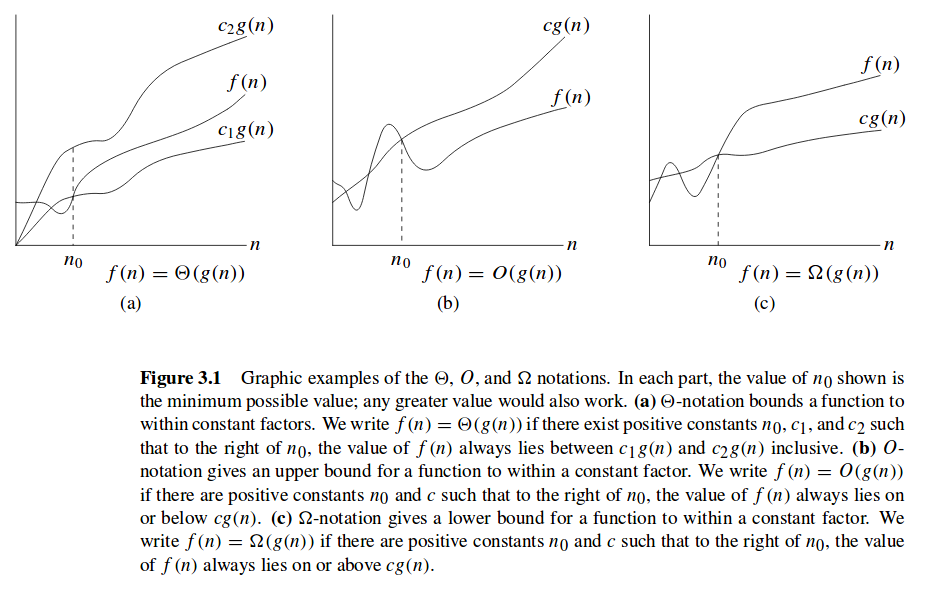
\includegraphics[width=0.9\textwidth]{graficos/complejidad.png}
\end{SCfigure}

\section{Notaci\'on $\Theta$}

Para una funci\'on $g(n)$ dada, notaremos a $\Theta(g(n))$ como el conjunto de funciones $f(n)$ que a partir de un numero $n_0 > 0$ sus valores pueden ser acotados entre $c_1g(n)$ y $c_2g(n)$ para alg\'un $c_1, c_2 \in \Re_{>0}$. Descripto formalmente quedar\'ia de la siguiente manera:

\begin{equation*}
 \Theta(g(n)) = \{ f(n) : (\exists\ c_1, c_2, n_0 \in \Re_{>0}) \ (\forall n\ |\ n_0 \leq n)\ 0 \leq c_1 \cdot g(n) \leq f(n) \leq c_2 \cdot g(n) \}
\end{equation*}

~

Como $\Theta(g(n))$ es un conjunto, podremos escribir ``$f(n) \in \Theta(g(n))$'' para indicar que $f(n)$ es un miembro de $\Theta(g(n))$, a veces escribiremos ``$f(n) = \Theta(g(n))$'' para expresar exactamente lo mismo.
~

\textbf{Propiedades de $\Theta$}:
\begin{enumerate}
 \item Para cualquier funci\'on $f$ se tiene que $f \in \Theta(f)$.
 \item $\Theta(f) = \Theta(g) \iff f \in \Theta(g) \iff g \in \Theta(f)$.
 \item S\'i $f \in \Theta(g) \land g \in \Theta(h) \implies f \in \Theta(h)$.
 \item S\'i $f \in \Theta(g) \land f \in \Theta(h) \implies \Theta(g) = \Theta(h)$.
 \item S\'i existe $\lim_{n \to \infty} \frac{f(n)}{g(n)} = k$, seg\'un los valores que tome $k$:
	\begin{enumerate}
	  \item S\'i $k \neq 0$ y $k < \infty$ entonces $\Theta(f) = \Theta(g)$.
	  \item S\'i $k = 0$ entonces $\Theta(g) \neq \Theta(f)$.
	\end{enumerate}
\end{enumerate}

\section{Notaci\'on $O$}

El conjunto $\Theta$ asint\'oticamente acota una funci\'on inferior y superiormente. Cuando solo tenemos una \textbf{cota asint\'otica superior}, usaremos el conjunto $O$. Para una funci\'on dada $g(n)$, denotaremos por $O(g(n))$ al conjunto de funciones tales que:

\begin{equation*}
 O(g(n)) = \{ f(n) : (\exists\ c, n_0 \in \Re_{>0}) \ (\forall n\ |\ n_0 \leq n)\ 0 \leq f(n) \leq c \cdot g(n) \}
\end{equation*}

~

Es decir que para todos los valores de $n$ a la derecha de $n_0$, el valor de la funci\'on $f(n)$ est\'a por debajo de $c \cdot g(n)$. Escribiremos $f(n) = O(g(n))$ para indicar que una funci\'on $f(n)$ es un miembro del conjunto $O(g(n))$. Notar que $f(n) = \Theta(g(n))$ implica $f(n) = O(g(n))$, ya que la noci\'on de $\Theta$ es mucho mas fuerte que la noci\'on de $O$. Esto es, escrito en forma de teor\'ia de conjuntos, que vale la inclusi\'on $\Theta(g(n)) \subseteq O(g(n))$

~

\textbf{Propiedades de $O$}:
\begin{enumerate}
 \item Para cualquier funci\'on $f$ se tiene que $f \in O(f)$.
 \item $f \in O(g) \implies O(f) \subset O(g)$.
 \item $O(f) = O(g) \iff f \in O(g) \land g \in O(f)$.
 \item S\'i $f \in O(g) \land g \in O(h) \implies f \in O(h)$.
 \item S\'i $f \in O(g) \land f \in O(h) \implies f \in O(min(g,h))$.
 \item S\'i existe $\lim_{n \to \infty} \frac{f(n)}{g(n)} = k$, seg\'un los valores que tome $k$:
	\begin{enumerate}
	  \item S\'i $k \neq 0$ y $k < \infty$ entonces $O(f) = O(g)$.
	  \item S\'i $k = 0$ entonces $f \in O(g)$, es decir, $O(f) \subset O(g)$, pero sin embargo se verifica que $g \notin O(f)$.
	\end{enumerate}
\end{enumerate}

\section{Notaci\'on $\Omega$}

De forma tal como la notaci\'on $O$ proporciona una cota asint\'otica en una funci\'on, $\Omega$ provee una \textbf{cota asint\'otica inferior}. Para una funci\'on dada $g(n)$, notaremos a $\Omega(g(n))$ como el conjunto de funciones tales que:

\begin{equation*}
 \Omega(g(n)) = \{ f(n) : (\exists\ c n_0 \in \Re_{>0}) \ (\forall n\ |\ n_0 \leq n)\ 0 \leq c \cdot g(n) \leq f(n) \}
\end{equation*}

~

Cuando decimos que el tiempo de un algoritmo es $\Omega(g(n))$, significa que no importa que particular entrada de tama\~no $n$ para cada valor de $n$, el tiempo que tardara el algoritmo con dicha entrara sera de al menos un numero constante de veces $g(n)$, para un $n$ suficientemente grande. Equivalentemente, esto nos da una cota temporal inferior para el mejor caso del algoritmo. De las definiciones de las notaciones asint\'oticas, es f\'acil ver que para cualquier dos funciones $f(n)$ y $g(n)$, tendremos que $f(n) = \Theta(g(n))$ si y solo si $f(n) = O(g(n))$ y $f(n) = \Omega(g(n))$. Usando una notaci\'on de teor\'ia de conjuntos esto seria equivalente a decir que $\Omega(g(n)) \cap O(g(n)) = \Theta(g(n))$, y si $f(n) \in \Omega(g(n)) \land f \in O(g(n))$ entonces $f(n)$ pertenecer\'a a ambos conjuntos, por lo que en particular pertenecer\'a a la intersecci\'on $\Theta(g(n))$.

~

\textbf{Propiedades de $\Omega$}:
\begin{enumerate}
 \item Para cualquier funci\'on $f$ se tiene que $f \in \Omega(f)$.
 \item $f \in \Omega(g) \implies \Omega(f) \subset \Omega(g)$.
 \item $\Omega(f) = \Omega(g) \iff f \in \Omega(g) \land g \in \Omega(f)$.
 \item S\'i $f \in \Omega(g) \land g \in \Omega(h) \implies f \in \Omega(h)$.
 \item S\'i $f \in \Omega(g) \land f \in \Omega(h) \implies f \in \Omega(max(g,h))$.
 \item $f(n) = \Omega(g(n)) \iff g(n) = O(f(n))$
 \item S\'i existe $\lim_{n \to \infty} \frac{f(n)}{g(n)} = k$, seg\'un los valores que tome $k$:
	\begin{enumerate}
	  \item S\'i $k \neq 0$ y $k < \infty$ entonces $\Omega(f) = \Omega(g)$.
	  \item S\'i $k = 0$ entonces $g \in \Omega(f)$, es decir, $\Omega(g) \subset \Omega(f)$, pero sin embargo se verifica que $g \notin \Omega(f)$.
	\end{enumerate}
\end{enumerate}

\textbf{Teorema:}
Para dos funciones cualesquiera f(n) y g(n), $f(n)= \Theta(g(n))$ si y solo si $f(n)= O(g(n))$ y $f(n)= \Omega(g(n))$



\newpage

\chapter{Dise\~no jer\'arquico de tipos de datos abstractos}

En la etapa de especificaci\'on de problemas, lo \'unico que hemos hecho es detallar qu\'e debemos hacer, pero no nos hemos preocupado por c\'omo hacerlo. El objetivo era describir el comportamiento del problema a resolver, pero no interesaba determinar c\'omo lo resolver\'iamos. Esto significa que al especificar estamos describiendo el problema, reci\'en al dise\~nar comenzamos a resolverlo.

\subsection{Dise\~no}

Al dise\~nar, centraremos nuestro inter\'es tanto en el \'ambito en el que ser\'a usado el tipo abstracto de datos como en los aspectos que se necesitan optimizar de este tipo, los cuales pueden estar dados por requerimientos expl\'icitos de eficiencia temporal o espacial. Sobre la base de esta informaci\'on, a la que llamaremos \textbf{contexto de uso}, dise\~naremos nuestro tipo aprovechando las ventajas que el contexto nos ofrezca y cuidando de responder a los requisitos que nos plantea.

En esta etapa, al buscarle representaciones menos abstractas al modelo especificado, es donde realmente comenzaremos a aprovechar el nivel de abstracci\'on. Cuanto m\'as abstracto sea el modelo, m\'as opciones de dise\~no tendremos disponibles en cada paso. B\'asicamente nuestra metodolog\'ia de dise\~no partir\'a entonces de un modelo abstracto no implementable directamente en un lenguaje imperativo de programaci\'on, y aplicar\'a iterativamente sobre dicho modelo sucesivos pasos de refinamiento hasta llegar a estructuras que si son implementables. En cada una de estas sucesivas iteraciones estaremos realizando, de cierta forma, una desabstracci\'on.

~

Es importante tener en cuenta que en la especificaci\'on estaremos centrados en un paradigma funcional y en la etapa de dise\~no nos centraremos en paradigma imperativo, por lo que tendremos un cambio de paradigma adem\'as de la desabstracci\'on del modelo, lo que nos conllevara ciertas dificultades. Uno de los objetivos del lenguaje de dise\~no es justamente permitir un cambio de paradigma que resulte ordenado.

\subsection{Jer\'arquico}

Cada iteraci\'on de desabstracci\'on de este proceso definir\'a un nivel de nuestro dise\~no. Por su parte, cada uno de estos niveles tendr\'a asociado uno o m\'as m\'odulos de abstracci\'on, que indicaran c\'omo se resuelven las operaciones de un m\'odulo utilizando otras operaciones de m\'odulos del nivel inmediato inferior. Cada uno de estos m\'odulos de abstracci\'on resultantes de cada iteraci\'on, ser\'a implementable en un lenguaje de programaci\'on, obteniendo de tal forma un dise\~no estratificado en niveles donde los m\'odulos de un cierto nivel son usuarios de los servicios que les brindan los del nivel inmediato inferior y no conocen (ni usan) a los m\'odulos de otros niveles. Un m\'odulo dar\'a a conocer los servicios que provee a trav\'es de una declaraci\'on de las operaciones que exporte junto con la aridad de cada una de ellas, se dar\'an a conocer las precondiciones (estado esperado de la m\'aquina antes de ejecutarse la operaci\'on) y las postcondiciones (como incidir\'a la ejecuci\'on en
el estado anterior). Esta informaci\'on estar\'a incluida en la interfaz del m\'odulo.

~

Esta separaci\'on o encapsulamiento en niveles provocara que cualquier cambio de implementaci\'on de nivel $n$ ser\'a transparente al nivel superior $n+1$, siempre que el nivel $n$ mantenga su interfaz. Esto es, que el m\'odulo exporte al menos las mismas funciones que se exportaban antes y la funcionalidad provista por las mismas no cambie, aunque puede haber mejorado su performance. Podremos verificar la validez del cambio de dise\~no viendo que la veracidad de las precondiciones y postcondiciones del nivel redise\~nado se mantiene con respecto a la versi\'on anterior.

\section{Lenguaje de dise\~no}

\subsection{Paradigma imperativo}

Para especificar formalmente el problema a resolver escrib\'iamos el tipo abstracto de datos siguiendo un paradigma funcional. Sin embargo al dise\~nar, debemos realizar un cambio de paradigma para poder expresar nuestra representaci\'on del modelo en un lenguaje imperativo, el cual se ajusta a los lenguajes de programaci\'on m\'as usados. En esta secci\'on discutiremos los principales aspectos que deberemos tener en cuenta al afrontar tal cambio.

\subsubsection*{Valores vs. Objetos}

Las aridades de las operaciones que definimos en la especificaci\'on para los tipos est\'an en una notaci\'on funcional, esto quiere decir que supone que las mismas construyen un objeto nuevo y lo devuelven a aquel que las llamo. Una caracter\'istica de esta notaci\'on es la \textit{transparencia referencial}, esto es que una expresi\'on siempre da el mismo resultado sin importar su contexto. En este paradigma, los datos s\'olo tienen sentido en cuanto sean argumentos o resultados de funciones.

Por otro lado, en el paradigma imperativo los datos son tratados como entidades independientes de las funciones que los utilizan. Es usual que se trabaje con una instancia de un objeto que se va modificando y cuyos valores anteriores no interesen. Por lo tanto, por cuestiones de optimizaci\'on y uso, no tiene sentido construir cada vez un objeto nuevo para devolverlo como resultado de una funci\'on, sino que en cambio se modificara el objeto original.

\subsubsection*{Par\'ametros que se modifican}

El mapeo de los par\'ametros de las funciones del TAD en las operaciones del m\'odulo no siempre es uno a uno. De hecho en el paradigma imperativo se acostumbra a modificar los par\'ametros como parte de respuesta del algoritmo y a devolver en el valor de retorno de la funci\'on, alg\'un estado que informe si la operaci\'on se completo de forma correcta o si hubo alg\'un problema. Esto nos brinda una mayor versatilidad a la hora de dise\~nar las interfaces, ya que una misma funci\'on puede devolver varios tipos de resultados sin necesidad de hacerlo mediante una tupla y adem\'as dar alguna informaci\'on acerca de la ejecuci\'on.

\subsection{Declaraci\'on de operaciones y pasaje de par\'ametros}

Para declarar las operaciones se le asignara un nombre, se describir\'an los argumentos y los tipos de cada uno como as\'i tambi\'en el tipo de dato del valor de retorno de la funci\'on. Para par\'ametro puede ser pasado a una funci\'on de 3 formas: entrada (\textbf{in}), salida(\textbf{out}) o entrada-salida (\textbf{in}/\textbf{out}).

Recordemos que en el paradigma imperativo todos los valores son pasados por referencia, exceptuando a los tipos primitivos (bool, nat, int, real, char, puntero) que son pasados por valor o copia$^*$. Al ser pasados por referencia y al ser del tipo de entrada-salida o salida y efectuar una asignaci\'on sobre el mismo, el valor con el que fue llamada la funci\'on es sobreescrito y el nuevo valor ser\'a el que mantendr\'a la variable luego de salir de la funci\'on, esto quiere decir que la variable que pasamos como par\'ametro de la funci\'on es efectivamente modificada por mas que nos encontremos dentro del scope de la funci\'on.

\subsection{Asignaci\'on y aliasing}

La expresi\'on $A \gets B$ (siendo $A$ y $B$ variables de un mismo tipo), denota la asignaci\'on del valor $B$ a la variable $A$. Esto funciona del mismo modo que el pasaje de par\'ametros. Si $A$ y $B$ pertenecen a un tipo primitivo $A$ pasara a ser copia de $B$, y si no son tipos primitivos, luego de haber efectuado la asignaci\'on, $A$ y $B$ har\'an referencia a la misma estructura f\'isica, es decir $A$ sera un alias de $B$ y viceversa (de ah\'i el nombre).

\section{Metodolog\'ia de dise\~no}

Nuestro objetivo es obtener un dise\~no jer\'arquico y modular. Para realizar esto hay varias formas pero presentaremos un m\'etodo que tiene las nociones de los distintos niveles en la jerarqu\'ia. Cada uno de los niveles tendr\'a asociado un m\'odulo de abstracci\'on. Para ser m\'as precisos, habr\'a distintos tipos abstractos de datos que deberemos dise\~nar, a cada uno de ellos le corresponder\'a un m\'odulo de abstracci\'on. A grandes rasgos, el m\'etodo se compone de los siguientes pasos:

\begin{itemize}
 \item Elecci\'on del tipo abstracto de datos a dise\~nar.
 \item Implementaci\'on del m\'odulo de abstracci\'on para el tipo abstracto de datos elegido.
 \item Iteraci\'on o finalizaci\'on.
\end{itemize}

\subsection{Elecci\'on del tipo a dise\~nar}

El orden en el cual se dise\~nan los tipos es arbitrario. Sin embargo es una buena pr\'actica comenzar por los tipos m\'as importantes, pues \'estos ser\'an los principales generadores de requerimientos de eficiencia para los tipos menos importantes o de niveles inferiores, aplicando un esquema top-down. Es importante notar que el proceso de dise\~no posee una natural ida y vuelta. Por ejemplo, la redefinici\'on de las funciones de un tipo puede obligarnos a reveer la secci\'on representaci\'on de un tipo que basa su dise\~no en \'este. Si lo vemos desde el punto de vista expl\'icitamente jer\'arquico, la redefinici\'on de las operaciones de un tipo de un nivel, puede obligarnos a redefinir a un modulo de un nivel superior.

\subsection{Implementaci\'on del m\'odulo de abstracci\'on para el tipo elegido}

Una vez elegido el tipo a dise\~nar, crearemos su m\'odulo de abstracci\'on correspondiente. El m\'odulo de abstracci\'on deber\'a describir de forma clara y concisa las operaciones que podr\'a realizar, como as\'i tambi\'en los efectos de las mismas sobre los datos, las complejidades temporales y espaciales que tomar\'an su uso y cuales de las operaciones podr\'an ser utilizadas externamente, es decir, cuales se exportar\'an. Adem\'as de dar una descripci\'on externa del mismo poseer\'a otra secci\'on en la cual se explicitar\'a la implementaci\'on de cada una de las operaciones (incluyendo operaciones privadas auxiliares) como as\'i tambi\'en la estructura de datos interna utilizada para llevar al cabo las tareas.

\subsection{Iteraci\'on o finalizaci\'on.}
En este punto tenemos un dise\~no que puede contener tipos para los que no tenemos una propuesta de dise\~no. En realidad son otros problemas a resolver de nivel de abstracci\'on menor al original. Por lo tanto, debemos volver a repetir el m\'etodo con los nuevos tipos a dise\~nar.La iteraci\'on prosigue hasta llegar a tipos que tengamos dise\~nados en nuestra biblioteca o sean primitivos.

\section{M\'odulo de abstracci\'on}

Cada m\'odulo de abstracci\'on est\'a compuesto por dos secciones: la \textbf{definici\'on de la interfaz} y la \textbf{definici\'on de la representaci\'on}. En la \textbf{interfaz} se describe la funcionalidad del m\'odulo y en qu\'e contexto puede ser usado. En la \textbf{representaci\'on} se elige, bajo alg\'un criterio, una forma de representaci\'on utilizando otros m\'odulos y se resuelven las operaciones del m\'odulo en funci\'on de su representaci\'on. Dicho de otra forma, se eligen las estructuras de datos internas que representar\'an el modulo y se implementan los algoritmos que la interfaz expresa. Un m\'odulo de dise\~no debe tener la siguiente estructura:

\begin{SCfigure}[1][ht!]
 \centering
 \includegraphics[width=0.7\textwidth]{graficos/ModuloDeDisenio.pdf}
\end{SCfigure}

\begin{itemize}
 \item \textbf{Especificaci\'on} Puede omitirse si es uno de los TADs provistos por la c\'atedra, o incluirse s\'olo los cambios si es una extensi\'on de un TAD ya conocido.
 \item \textbf{Interfaz} La cual contendr\'a los servicios exportados, \'ordenes de complejidad, aspectos de aliasing, efectos secundarios, etc. En definitiva, todo lo que el usuario necesite saber.
 \item \textbf{Representaci\'on} Estructura interna, invariante, funci\'on de abstracci\'on y algoritmos.
 \item \textbf{Servicios usados} \'Ordenes de complejidad, aspectos de aliasing, etc. requeridos de los tipos de soporte que utilizamos en nuestro m\'odulo.
\end{itemize}


\subsection{Aspectos de la Interfaz}

En este paso tomamos las decisiones concernientes al cambio de paradigma. Una forma de lograr esto es redefinir las aridades de las funciones adapt\'andolas a un lenguaje imperativo explicitando los requerimientos (precondiciones) para la aplicaci\'on de cada operaci\'on y los efectos que tiene sobre el estado de la m\'aquina (postcondiciones). Para escribir las precondiciones y las postcondiciones usaremos un lenguaje de descripci\'on de estados aprovechando la especificaci\'on del tipo a dise\~nar.

\subsubsection{Servicios exportados / Operaciones exportadas}

En esta secci\'on deben estar expresados los detalles acerca de nuestro m\'odulo que resulten indispensables a sus usuarios. Es imprescindible tocar temas como la complejidad temporal de los algoritmos y cuestiones de aliasing y efectos secundarios de las operaciones. Adem\'as, pueden exhibirse comentarios (a modo informativo) con respecto a la implementaci\'on del m\'odulo que, aunque tengan menor importancia, sean de inter\'es para el usuario.

\subsubsection{Relaci\'on entre el dise\~no y la especificaci\'on, precondiciones y postcondiciones}

Al describir la interfaz de un m\'odulo para cada una de las operaciones deberemos indicar cu\'ales son sus restricciones y qu\'e efectos produce en el estado de la m\'aquina. Para describir esto haremos uso de la especificaci\'on del tipo abstracto de datos asociado al m\'odulo, lo que en consecuencia nos obligar\'a a describir la relaci\'on que existe entre las variables del dise\~no y el tipo abstracto de datos especificado. Queremos poder describir en la interfaz cual es el resultado final luego de aplicada una operaci\'on teniendo en cuenta los par\'ametros con los cuales se la invoca y las relaciones entre ellos.

~

Cuando nos pasa esto tenemos el problema de que los tipos y operaciones a las que queremos hacer referencia est\'an en el mundo de los TADs y por otro lado, las funciones sobre las que queremos describir su entrada y resultado est\'an en el mundo del dise\~no. Por lo que de cierta forma queremos comparar elementos que no est\'an definidos en base a axiomas, con elementos que si lo est\'an. Para subsanar esta dificultad, existir\'a la funci\'on $\widehat{\text{\textbullet}}$.

~

Llamaremos $G_I$ al conjunto de g\'eneros del paradigma imperativo y $G_F$ al conjunto de g\'eneros del paradigma funcional. Sub-indexaremos con $I$ a los g\'eneros de $G_I$ y con $F$ a los de $G_F$. Es decir, disponemos de una funci\'on que dado un g\'enero del paradigma imperativo nos da su ``equivalente'' en el paradigma funcional, la misma quedara definida como:

\begin{equation*}
 \widehat{\text{\textbullet}}: G_I \rightarrow G_F
\end{equation*}

Mediante el uso de esta funci\'on podremos establecer de forma clara el mapeo entre las operaciones del m\'odulo y las funciones de la especificaci\'on cuando escribamos las precondiciones y postcondiciones de cada operaci\'on del m\'odulo.

\subsection{Aspectos de la Implementaci\'on}

El objetivo de esta secci\'on es definir la forma en que representaremos el tipo que estamos dise\~nando en esta iteraci\'on (o nivel). La elecci\'on de una forma de representaci\'on est\'a dada por la elecci\'on de una o m\'as estructuras, las cuales deber\'an estar debidamente justificadas. Adem\'as de elegir la estructura de representaci\'on, es necesario definir cu\'al es la relaci\'on entre la estructura de representaci\'on y el tipo representado. Por \'ultimo, se deber\'an proveer los algoritmos que operan sobre la estructura y que resuelven cada una de las operaciones.

La estructura de representaci\'on de las instancias de los tipos s\'olo ser\'a accesible (modificable, consultable) a trav\'es de las operaciones que se hayan detallado en la interfaz del m\'odulo de abstracci\'on respectivo. Las operaciones no exportadas tambi\'en tendr\'an acceso a esta informaci\'on, pero s\'olo podr\'an ser invocadas desde operaciones del mismo m\'odulo, es decir la visibilidad de las mismas fuera del m\'odulo ser\'a nula.

\subsubsection{Elecci\'on de la estructura de representaci\'on} %Relacionado con Contexto de uso y requerimientos de eficiencia de los servicios prestados, hay que unificar.

La elecci\'on de la estructura esta fundamentada sobre las operaciones que nos interesa optimizar y el contexto de uso en el que ser\'an utilizadas. No solo tomamos en cuenta la complejidad temporal para definir un criterio de optimizaci\'on sino que tambi\'en tomamos en cuenta el espacio de disco, espacio en memoria, reusabilidad, claridad, sencillez de la implementaci\'on, homogeneidad de los algoritmos, entre otros.

Las variables en un programa referencian valores. Ser\'a imposible el acceso a la representaci\'on interna de \'estos y esto redundar\'a en la modularidad de nuestro dise\~no y en el ocultamiento de la informaci\'on. El ocultamiento nos permite hacer invisibles algunos aspectos que ser\'an encapsulados. Esto es \'util para aumentar el nivel de abstracci\'on y dise\~nar c\'odigo que sea m\'as f\'acilmente modificable, mantenible y extensible. Al acceder a los objetos s\'olo a trav\'es de su interfaz no nos atamos a su implementaci\'on, s\'olo a su funcionalidad.

\subsubsection{Relaci\'on entre la implementaci\'on y la abstracci\'on}

Para poder relacionar el mundo de los TADs con el mundo del dise\~no haremos uso de dos funciones que nos facilitaran esta tarea. Ambas funciones tendr\'an su dominio en las instancias de representaci\'on, estas son todas las formas que tendremos de instanciar la estructura de datos que elegimos en la representaci\'on sin restricci\'on alguna. Como podremos imaginar, muchas de estas formas de instancias la representaci\'on no tendr\'an sentido alguno para el tipo que estamos representando, mas que nada si las variables de nuestra representaci\'on tienen alguna correlaci\'on (por ejemplo, cantidad de elementos y la lista con dichos elementos), es aqu\'i en donde \textbf{invariante de representaci\'on} cobrar\'a importancia, ya que es el que nos indicara que instancias de la representaci\'on tienen sentido para el tipo abstracto que estamos representando y cuales no. Luego, la \textbf{funci\'on de abstracci\'on} servir\'a para llevar una instancia de representaci\'on al mundo de los TADs, es decir a una instancia del tipo abstracto de datos que estamos representando.

\subsubsection{Invariante de representaci\'on}

\begin{equation*}
Rep: \widehat{\text{genero\_de\_representacion}} \rightarrow boolean
\end{equation*}

El invariante de representaci\'on es un predicado que nos indica si una instancia de la estructura de representaci\'on es v\'alida para representar una instancia del tipo representado. De cierta forma, es el conocimiento sobre la estructura que necesitan las distintas operaciones para funcionar correctamente y que garantizan las mismas al finalizar su ejecuci\'on. Adem\'as funciona como un concepto coordinador entre las operaciones. En \'el quedan expresados las restricciones de coherencia de la estructura, surgidas de la redundancia de informaci\'on que pueda haber.
Su dominio es la imagen funcional del tipo que estamos implementando, lo cual es necesario para que podamos ``tratar'' los elementos del dominio en l\'ogica de primer orden.

Todas las \textbf{operaciones exportadas} del tipo deber preservar el invariante de representaci\'on. Las \textbf{operaciones auxiliares} o internas, es decir aquellas que no aparecen en la interfaz y por lo tanto son invisibles a factores externos del m\'odulo, no tienen la necesidad conservar el invariante, ser\'a nuestra responsabilidad conocer que modificaciones le realizan a la estructura interna (de hacerlas) para luego restaurar el invariante.

De cierta forma, el invariante de representaci\'on fuerza a las operaciones a cumplir ciertos ordenes de complejidad y a preservar la coherencia en la estructura de representaci\'on. Adem\'as al ser un predicado que debe cumplirse gran parte del tiempo, podremos deducir propiedades del mismo que podremos usar como parte de nuestras demostraciones de correctitud y complejidad.

\subsubsection{Funci\'on de abstracci\'on}

\begin{equation*}
 Abs: \widehat{\text{genero\_de\_representacion}}\ g \rightarrow \widehat{\text{genero\_del\_tipo\_abstracto\_representado}} \ \ \ \ \{Rep(g)\}
\end{equation*}

La funci\'on de abstracci\'on es una herramienta que permite vincular una estructura de representaci\'on con el valor abstracto al que representa, es decir con el TAD vinculado al m\'odulo de abstracci\'on. Tiene por dominio al conjunto de instancias que son la imagen abstracta del tipo de representaci\'on (al igual que el invariante de representaci\'on) y que adem\'as verifican el invariante de representaci\'on, por esto mismo la funci\'on sera sobreyectiva. La funci\'on devuelve una imagen abstracta de la instancia del tipo representado (aquella instancia que estamos pretendiendo representar del tipo abstracto) y diremos que $T$ representa a $A$ si $Abs(\widehat{T})=_{obs} A$, en donde $T$ es una instancia de la representaci\'on y $A$ una instancia del TAD. Informalmente la funci\'on de abstracci\'on cumple la funci\'on de verificar que las funciones que alteran la estructura de representaci\'on realicen lo que est\'a especificado en el TAD y no otra cosa.

\begin{SCfigure}[1][ht!]
 \centering
 \includegraphics[width=0.3\textwidth]{graficos/FuncionDeAbstraccion.pdf}
 \caption*{\footnotesize $A$ ser\'a el modulo en cuesti\'on que estaremos dise\~nando y $B$ la estructura de representaci\'on del mismo. El circulo con el punto dentro hace alusi\'on al hecho de que la conmutaci\'on del triangulo conserva la sanidad. Esto significa que la aplicaci\'on de la funci\'on de abstracci\'on a $B$ deber\'a dar el mismo resultado que la aplicaci\'on de $\widehat{\text{\textbullet}}$ a $A$.
 \newline
 \newline }
\end{SCfigure}

Tendremos dos formas de describir la funci\'on de abstracci\'on. La primera de ellas, en funci\'on de sus observadores b\'asicos. Dado que los observadores identifican de manera un\'ivoca al objeto del cual hablan, si nosotros describimos el valor que tienen los observadores b\'asicos una vez aplicados al objeto, estaremos describiendo desde un punto observacional pero sin ambig\"uedad el objeto representado. Otra forma de describir la funci\'on de abstracci\'on es utilizando los generadores del tipo de representaci\'on. La elecci\'on de elegir una forma u otra de hacerlo depende de la comodidad y declaratividad.

Dicho de otra forma, el objetivo de la funci\'on de abstracci\'on es poner en consonancia el tipo de soporte del modulo abstracto con los observadores del tipo que esta siendo representado. Una de las formas de realizar esto es caracterizando el valor de todos los observadores del TAD en base a valores de la instancia de la estructura de representaci\'on, de esa forma obtiene una instancia del TAD en consonancia con el modulo abstracto.


\newpage

\chapter{Estructuras de Datos}

\section{Estructuras b\'asicas}
\subsection{Lista}
\subsection{Cola}

La estructura Cola se puede pensar como un arreglo para guardar los elementos m\'as un natural para saber la cantidad. Las colas se caracterizan por ser una estructura de tipo FIFO (First in, First out. O en castellano: Primero que entra, primero que sale).
Una implementaci\'on efectiva de una Cola puede hacerse usando \textbf{Aritmetica Circular}, alias: funci\'on m\'odulo. Idea:
\begin{enumerate}
 \item Tengo un arreglo de MAX\_CANTIDAD elementos.
 \item En una variable \textit{cant} guardo la cantidad de elementos actuales en la cola.
 \item En una variable \textit{primero} guardo la posici\'on en el arreglo del primer elemento.
 \item Encolar: agrega el nuevo elemento a la posici\'on $(primero + cant) \% MAX\_CANTIDAD$ del arreglo e  incrementa \textit{cant} en uno.
 \item Desencolar: setea $primero=(primero + 1) \% MAX\_CANTIDAD$ y decrementa \textit{cant} en uno.
\end{enumerate}
Siendo las complejidades resultantes:
\begin{itemize}
 \item \textbf{Pr\'oximo} $O(1)$
 \item \textbf{Desencolar} $O(1)$
 \item \textbf{Encolar} $O(1)$
 \item \textbf{B\'usqueda} $O(n)$
\end{itemize}
Una clara limitaci\'on de \'esta implementaci\'on es que solo puede almacenar hasta MAX\_CANTIDAD elementos al mismo tiempo. Se puede resolver esto y agregar algunas ventajas utilizando \textbf{Memoria Din\'amica}.

\subsection{Pila}
\subsection{Arreglo dimensionable}

\newpage
\section{\'Arboles}
\subsection{\'Arbol binario de b\'usqueda}

Un \'arbol binario de b\'usqueda es un \'arbol basado en nodos binarios el cual puede ser representado por una estructura de punteros en donde cada nodo es un objeto. En adici\'on a la clave y a los datos, cada nodo contiene los atributos izquierda, derecha y p, los cuales son punteros que apuntan a su hijo izquierdo, hijo derecho y padre, respectivamente. Si un hijo o un padre esta perdido el atributo apropiado contiene el valor $NIL$. El nodo ra\'iz es el \'unico nodo cuyo padre es $NIL$.

Las claves en un \'arbol binario de b\'usqueda siempre est\'an guardadas de forma tal de satisfacer la \textbf{invariante del \'arbol binario de b\'usqueda}, el cual se define como: ''Sea $x$ un nodo en un \'arbol de b\'usqueda binario. Si $y$ es un nodo en el sub-\'arbol izquierdo de $x$, entonces $y.clave \leq x.clave$. Si $y$ es un nodo en el sub-\'arbol derecho de $x$, entonces $y.clave \geq x.clave$``

\subsubsection{B\'usqueda}

La b\'usqueda en un \'arbol binario se logra utilizando el invariante presentado anteriormente. El procedimiento comienza en la ra\'iz y por cada nodo $x$ que encuentra compara la clave $k$ con $x.clave$, si las dos claves son iguales, la b\'usqueda termina. Si $k$ es mas chico que $x.clave$, la b\'usqueda continua por el sub-\'arbol izquierdo de $x$, dado que el invariante del \'arbol binario de b\'usqueda implica que $k$ no puede ser guardado en el sub-\'arbol derecho. Sim\'etricamente, si $k$ es mas grande que $x.clave$, la b\'usqueda continua por el sub-\'arbol derecho. Los nodos encontrados durante la recursi\'on forman un camino simple desde la ra\'iz, por lo que el tiempo de corrida de una b\'usqueda en un \'arbol binario es de $O(h)$, en donde $h$ es la altura del \'arbol la cual puede ser $n$ si tenemos un \'arbol totalmente degenerado, que de cierta forma terminar\'ia siendo una lista enlazada.

Adem\'as, siempre podremos encontrar un elemento en un \'arbol binario cuya clave sea un m\'inimo o un m\'aximo siguiendo los punteros izquierdos o derechos desde la ra\'iz hasta que encontremos un $NIL$.

\subsubsection{Inserci\'on}

Las operaciones de inserci\'on y borrado causa que la din\'amica del conjunto representado por un \'arbol binario de b\'usqueda cambie. La estructura de datos debe ser modificada para reflejar este cambio, pero de forma tal que el invariante se conserve.

Para insertar un nuevo valor $v$ en un \'arbol binario de b\'usqueda $T$, crearemos un nuevo nodo $z$ de tal forma que $z.clave = v$, $z.izq = NIL$ y $z.der = NIL$. Modificara $T$ y alguno de los atributos de $z$ de tal forma que inserte $z$ en la posici\'on apropiada del \'arbol. Para lograr insertar el nuevo nodo el procedimiento guardar\'a en una variable $p$ un puntero al nodo actual en donde se encuentra mientras que ejecuta una b\'usqueda en el \'arbol. Una vez que llega a un nodo NIL durante la b\'usqueda, asigna $z.p = p$ y compara $z.clave$ con $p.clave$, si es mayor asigna $p.izq = z$ y si es menor $p.der = z$, de esta forma el invariante queda restaurado. El tiempo de esta operaci\'on se encontrara en el orden de $O(h)$, siendo que $h$ puede ser $n$ en el peor caso el tiempo ser\'a de $O(n)$, sin embargo el caso promedio suponiendo una distribuci\'on uniforme en la entrada de los valores sera de $O(lg(n))$.

\subsubsection{Borrado}

La estrategia general para eliminar un nodo $z$ de un \'arbol binario de b\'usqueda $T$ tiene $3$ casos b\'asicos, pero como veremos uno de ellos es algo enga\~noso.

\begin{itemize}
 \item Si $z$ no tiene hijos, entonces simplemente lo removeremos modificando su padre $z.p$ reemplazando el puntero a $z$ por $NIL$.
 \item Si $z$ solo tiene un hijo, entonces \textbf{elevaremos} dicho hijo para tomar la posici\'on de $z$ modificando el padre $z.p$ reemplazando el puntero a $z$ por el puntero al \'unico hijo de $z$.
 \item Si $z$ tiene dos hijos, entonces encontraremos el m\'inimo $y$ en el sub-\'arbol derecho de $z$ (es decir, su sucesor), para tomar la posici\'on de $z$ en el \'arbol. Como $y$ era el m\'inimo del sub-\'arbol derecho de $z$, $y.izq$ sera $NIL$ y si $y$ tiene un hijo izquierdo lo elevaremos al padre de $y$. Luego, con $y$ libre hijos, lo reemplazaremos por $z$ y le asignaremos los sub-\'arboles derecho e izquierdo, como hijos de $y$. Esto mismo se puede hacer si tomamos como $y$ el m\'aximo del sub-\'arbol izquierdo de $z$.
\end{itemize}

\subsubsection{Balanceo perfecto}

Vimos que los ABB funcionan razonablemente bien en el caso promedio, pero no dan garant\'ias. Todos los algoritmos que vimos tienen un peor caso lineal. En \'este sentido, los arreglos tambi\'en son lineales en el peor caso, pero ocupan menos memoria.

Pero si miramos en detalle, veremos que los algoritmos m\'as bien son $O(h)$, donde $h$ es la altura del \'arbol. Entonces, s\'i distribuy\'esemos los nodos del ABB de manera ``pareja'', de manera tal que el \'arbol tuviese la m\'inima altura y estuviese siempre parejo, obtendr\'iamos unas complejidades mucho mejores.

~

\textbf{Teorema}: un \'arbol binario perfectamente balanceado de $n$ nodos (no nil, es decir $n>0$) tiene altura $\lfloor log_2 n \rfloor + 1$.

~

Supongamos que cada nodo tiene 0 o 2 hijos. Llamemos $n_i$ a la cantidad de nodos internos (m\'as la raiz) y $n_h$ a la cantidad de hojas.

~

\textit{Propiedad}: Si $n > 1$, $n_h = n_i + 1$

El caso base es trivial. $n = 3$ (raiz con dos hijos) $\implies n_h = 2 \land n_i = 1$ (la raiz). Entonces se cumple la propiedad.

Para el paso inductivo, supongamos que vale para $n_h$ y $n_i$. Ahora, agreguemos un nivel al arbol. Las hojas se duplican, $n_h' = 2n_h$ y los nodos internos crecen en tantos como antes ten\'ia hojas:
$n_i' = n_i + n_h$, por hip\'otesis inductiva: $n_i' = (n_h - 1) + n_h = 2n_h - 1 = n_h' - 1$. $\square$

\textit{Corolario}: al menos la mitad de los nodos son hojas.

~

Luego, sabemos que (1) $n' = n_i' + n_h'$ y (prop) s\'i $n > 1$, $n_h = n_i + 1$. Imaginemos que podamos las hojas: nos queda un \'arbol (llamemos $n$ a la cantidad de nodos) con las mismas propiedades, 1 menos de altura (llam\'emosla $h$), la mitad de los nodos y ahora todas las ramas de la misma longitud. ¿Cu\'antas veces m\'as podemos podarlo? O dicho de otra forma: ¿Cu\'antos niveles se pueden agregar desde el comienzo para tener un \'arbol de altura $h$?

Al agregar un nivel, la cantidad de nodos se duplica, porque $n_h' = n_i' + 1$, pero $n_i' = n$, entonces $n_h' = n +1$. Reemplazando en (1) nos queda que $n' = n + (n + 1) + 1$. Entonces $n = 1 $.$ 2 \dots 2 = 2^h = 2^{log_2 n}$.
Por ende, $h = log_2n$ y la altura del \'arbol era $h+1$. $\square$

~

Conclusi\'on, s\'i tuvi\'esemos \'arboles perfectamente balanceados todas nuestras operaciones ser\'ian $O(log\ n)$. Pero mantener un balanceo perfecto es muy costoso, por lo que no es factible.
Sin embargo, podemos tener un balanceo ``casi'' perfecto, haciendo que todas las ramas tengan ``casi'' la misma longitud, donde ese ``casi'' lo vamos a interpretar de la siguiente manera: la longitud entre dos ramas cualesquiera de un nodo difiere a lo sumo en 1.

\'Esta clase de ABBs, son los llamadas \'arboles AVL.

\subsubsection{Rotaciones}

Las rotaciones son operaciones locales en un \'arbol de b\'usqueda que cambian la estructura de punteros del mismo preservando el invariante del \'arbol binario, son mayormente usadas en las distintas implementaciones de \'arboles balanceados para ajustar los factores de balanceo del mismo. Usaremos dos tipos de rotaciones, rotaciones hacia la izquierda y rotaciones hacia la derecha. Cuando hacemos una rotaci\'on hacia la izquierda en un nodo $x$, asumimos que su hijo derecho $y$ no es $NIL$; $x$ podr\'a ser cualquier nodo en el \'arbol cuyo hijo derecho no es $NIL$. La rotaci\'on hacia la izquierda ''pivotea`` alrededor del enlace de $x$ a $y$ y hace a $y$ la nueva ra\'iz del sub-\'arbol, dejando como hijo izquierdo de $y$ a $x$ y trasladando a el hijo izquierdo de $y$ al lugar del hijo derecho de $x$.

\begin{SCfigure}[1][ht!]
 \centering
 \includegraphics[width=0.7\textwidth]{graficos/RBRotacionIzq.pdf}
 \caption*{\newline \footnotesize Si nos imaginamos la rotaci\'on como bolillas e hilos, ''tirar\'iamos`` $y$ hacia arriba a la izquierda, haciendo que $x$ baje y quede a la altura del hijo izquierdo de $y$. Luego, como el hijo izquierdo de $y$ se encontraba en el sub-\'arbol derecho de $x$, sera mas grande que $x$, por lo que lo podremos asignar como hijo derecho de $x$.}
\end{SCfigure}

\subsubsection{Recorrido de \'arboles}

El recorrido de \'arboles, en ingles \textit{Tree traversal}, se refiere al proceso de visitar de manera sistem\'atica, exactamente una vez, a cada nodo de un \'arbol. Tales recorridos est\'an clasificados en el orden en el cual son visitados los nodos:

\textbf{Preorden (o ``preorder'')}: (ra\'iz, izquierdo, derecho). Comenzando con el nodo ra\'iz:
\begin{itemize}
 \item Visitar la raiz.
 \item Recorrer el sub\'arbol izquierdo en preorden.
 \item Recorrer el sub\'arbol derecho en preorden.
\end{itemize}

\textbf{Inorden (o ``inorder'')}:  (izquierdo, ra\'iz, derecho). Comenzando con el nodo ra\'iz:
\begin{itemize}
 \item Recorrer el sub\'arbol izquierdo en inorden.
 \item Visitar la raiz.
 \item Recorrer el sub\'arbol derecho en inorden.
\end{itemize}

\textbf{Postorden (o ``postorder'')}:  (izquierdo, derecho, ra\'iz). Comenzando con el nodo ra\'iz:
\begin{itemize}
 \item Recorrer el sub\'arbol izquierdo en postorden.
 \item Recorrer el sub\'arbol derecho en postorden.
 \item Visitar la raiz.
\end{itemize}

\subsubsection{Complejidades}

\begin{itemize}
 \item \textbf{B\'usqueda} $O(n)$ (caso promedio $O(lg(n))$)
 \item \textbf{Inserci\'on} $O(n)$ (caso promedio $O(lg(n))$)
 \item \textbf{Borrado} $O(n)$ (caso promedio $O(lg(n))$)
 \item \textbf{Espacio} $O(n)$
\end{itemize}

\subsection{Heap}

La estructura de datos del heap (binario) es un arreglo de objetos que representa una Cola de Prioridad y que podremos ver como un \'arbol binario casi-completo. Cada nodo del \'arbol corresponde a un elemento del arreglo y el \'arbol esta completamente lleno en todos los niveles excepto en el ultimo, el cual esta lleno desde la izquierda hasta alg\'un punto. Un arreglo $A$ que representa un heap es un objeto con dos atributos, $A.lenght$ que nos dir\'a la cantidad de elementos en el arreglo y $A.heap\_size$ que representara cuantos elementos en el heap est\'an guardados en el arreglo $A$. Esto es, que a pesar que $A[1..A.length]$ contenga n\'umeros, solo los elementos en $A[1..A.heap\_size]$ (en donde $0 \leq A.heap\_size \leq A.length$) son elementos validos del heap.

~

La ra\'iz del \'arbol estar\'a situada en $A[1]$, y dado el \'indice $i$ de un nodo, f\'acilmente podremos computar los \'indices de su padre, hijo derecho e izquierdo. El c\'omputo del \'indice del padre estar\'a definido de la forma $Padre(i) = \lfloor i/2 \rfloor$, mientras que los \'indices de los hijos podr\'an ser computados de la forma $Izquierda(i) = 2i$ y $Derecha(i) = 2i+1$, en donde $i \in [1..A.heap\_size]$. Hay dos tipos de heaps binarios, max-heaps y min-heaps. En ambos casos, los valores de los nodos satisfacen el invariante del heap, el cual depende del tipo de heap con el que trabajemos. En un max-heap, el invariante del max-heap nos dice que para cada nodo $i$ que no sea la ra\'iz se debe cumplir que $A[Padre(i)] \geq A[i]$, esto es que el valor de un nodo debe ser como m\'aximo el valor de su padre. Entonces, el m\'aximo en un max-heap estar\'a guardado en la ra\'iz, y el sub-\'arbol con ra\'iz en un nodo no podr\'a contener valores mas grandes que el nodo en si mismo. Un min-heap esta
organizado de la forma opuesta, el invariante de min-heap nos dice que para cada nodo $i$ distinto de la ra\'iz se debe cumplir $A[Padre(i)] \leq A[i]$, por lo que el elemento m\'inimo de un min-heap estar\'a en la ra\'iz.

~

Viendo el heap como un \'arbol, definiremos la altura de un nodo en un heap como el numero de aristas en el camino simple mas largo desde el nodo mismo hasta una hoja, y definiremos la altura del heap como la altura de su ra\'iz. Ya que un heap de $n$ elementos esta basado en un \'arbol binario completo, su altura pertenecer\'a a $\Theta(lg(n))$.

\subsubsection{Mantener el invariante del heap}

De aqu\'i en mas, asumiremos que estaremos hablando de un max-heap, ya que el min-heap es an\'alogo. Para mantener el invariante del max-heap en un arreglo, llamaremos al procedimiento \textbf{Heapify}. Su entrada sera el arreglo $A$ y un \'indice $i$ del arreglo. Cuando es llamado, Heapify asume que los sub-\'arboles binarios con sus ra\'ices en $Izquierda(i)$ y $Derecha(i)$ ser\'an max-heaps, pero que $A[i]$ puede ser mas chico que que sus hijos, violando as\'i el invariante. Heapify deja que el valor en $A[i]$ ''decante`` en el max-heap, de forma tal que el sub-\'arbol con ra\'iz en $i$ cumpla el invariante del heap y luego recursivamente se asegurara que el invariante sea cumplido en el sub-\'arbol en donde el valor $A[i]$ haya decantado.

~

Puntualmente lo que realiza Heapify es, estando situado en $i$, compara el valor con los valores de los hijos de $i$. Si ninguno de los valores de los hijos es mas grande que el valor de $i$ lo deja como esta, en el caso contrario intercambia el valor de $i$ con el valor de su hijo mas grande. Si bien en el nodo original el invariante se cumple, el invariante puede ser violado en el sub-\'arbol cuya ra\'iz fue intercambiada por lo que se realiza una llamada recursiva utilizando como $i$ el nuevo \'indice donde el valor fue intercambiado.

~

El tiempo de Heapify en un sub-\'arbol de tama\~no $n$ con su ra\'iz en un nodo $i$ sera el tiempo $\Theta(1)$ para ajustar las relaciones entre los elementos $A[i]$, $A[Izquierda(i)]$ y $A[Derecha(i)]$, mas el tiempo que tome correr Heapify en un sub-\'arbol con su ra\'iz en alguno de los hijos del nodo $i$ (asumiendo que la llamada recursiva ocurra). El peor caso ocurrir\'a cuando el nivel inferior del \'arbol se encuentre exactamente a la mitad de estar lleno, por lo que cada uno de los sub-\'arboles de los hijos tendr\'an como mucho $2n/3$ elementos. Podremos describir el tiempo de Heapify con la recurrencia $T(n) \leq T(2n/3) + \Theta(1)$. Si tuvi\'esemos $T(n) = T(2n/3) + \Theta(1)$, la recurrencia se ajusta al segundo caso del teorema maestro, por lo que $T(n) \subseteq \Theta(lg(n))$ pero como tenemos una relaci\'on de menor o igual en la recurrencia original, $T(n) \subset O(lg(n))$.

\subsubsection{Construyendo un heap (Algoritmo de Floyd)}

Podremos usar el procedimiento Heapify de forma bottom-up para convertir un arreglo $A[1..n]$, en donde $n=A.length$, en un max-heap. Los elementos en el sub-arreglo $A[\lfloor n/2\rfloor + 1 .. n]$ son todas hojas del \'arbol, y por lo tanto cada uno es un heap de $1$ elemento por el cual podremos comenzar. El procedimiento para construir un heap va por cada uno de los nodos del \'arbol restantes comenzando por el \'indice mas grande, es decir $i = \lfloor A.length/2 \rfloor .. 1$, y ejecuta Heapify en cada uno de ellos. Una cota grosera para este procedimiento es $O(nlg(n))$, ya que har\'a $n$ llamadas a Heapify. Sin embargo, una cota mas ajustada puede ser dada bas\'andonos en que la altura de un \'arbol heap de $n$ elementos tiene altura $\lfloor lg(n) \rfloor$ y como mucho $\lceil n/2^{h+1}\rceil$ nodos de cualquier altura $h$, la cual corresponder\'a con $O(n)$.

%TODO: Dar la demostracion de esto. Pagina 157 del cormen.

\subsubsection{Extraccion de m\'aximo e inserci\'on}

El m\'aximo en un max-heap sera $A[1]$, el cual una vez extra\'ido no ser\'a eliminado del arreglo sino que ser\'a intercambiado por el ultimo elemento del arreglo y luego se decrementara $A.heap\_size$ en una unidad, dejando fuera del scope al ultimo elemento del arreglo que ser\'a aquel que acabamos de extraer. El \'unico problema con esto es que estaremos rompiendo el invariante del heap, pero para solucionarlo solo nos bastara con aplicar $Heapify(A,1)$ ya que el resto de los sub-heaps seguir\'an siendo validos. Como todas las operaciones son $\Theta(1)$ exceptuando Heapify, la cual se usar\'a una sola vez, el tiempo total del algoritmo sera de $O(lg(n))$.

%TODO: Pseudocodigo de extraccion, pagina 163 del cormen

~

Para insertar un nuevo elemento incrementaremos la variable $A.heap\_size$ en una unidad y asignaremos el nuevo valor a la ultima posici\'on valida para el heap, es decir $A[heap\_size] = valor$. Luego, intercambiaremos su valor con el padre hasta que el invariante del heap se cumpla.

%TODO: Pseudocodigo de inserci\'on, pagina 164 del cormen.

\subsubsection{En resumen}

Los heaps son \'arboles balanceados en donde la clave de cada nodo es mayor o igual que la de sus hijos y en donde todo sub-\'arbol es un heap. Adicionalmente puede o no cumplir que por la forma de su implementaci\'on sea izquierdista, esto quiere decir que el \'arbol estar\'a todo lleno exceptuando su ultimo nivel, el cual se llenara de izquierda a derecha.

Su representaci\'on podr\'a estar dada por cualquier tipo de estructura para \'arboles binarios, pero si bien sera mas eficiente si se lo representa en un arreglo, pasaremos a una representaci\'on est\'atica por lo que podremos perder tiempo agrandando un arreglo. Sea un nodo $v$, la posici\'on dentro de un heap se calcula:

\begin{itemize}
 \item Si $v$ es la ra\'iz, $P(v) = 1$
 \item Si $v$ es un nodo que no es la ra\'iz, su padre $u$ sera $P(v) = \lfloor P(u)/2\rfloor$. Sea $i$ un \'indice de un nodo: $Padre(i) = \lfloor i/2\rfloor$.
 \item Si $v$ es un hijo izquierdo de $u$ $P(v) = 2P(u)$. Sea $i$ un \'indice de un nodo: $Derecho(i) = 2i$.
 \item Si $v$ es un hijo derecho de $u$ $P(v) = 2P(v)+1$. Sea $i$ un \'indice de un nodo: $Izquierdo(i) = 2i+1$.
\end{itemize}

\subsubsection{Complejidades}
Las complejidades de las operaciones del heap quedaran de la forma:

\begin{itemize}
 \item \textbf{Ver el m\'aximo o m\'inimo / Pr\'oximo} $O(1)$
 \item \textbf{Extraer el m\'aximo o m\'inimo / Desencolar} $O(lg(n))$
 \item \textbf{Ingresar nuevo elemento / Encolar} $O(lg(n))$
 \item \textbf{Construir heap a partir de arreglo / Heapify} $O(n)$
\end{itemize}

\subsection{\'Arbol balanceado en altura (AVL)}

Un \'arbol AVL es un \'arbol binario de b\'usqueda que esta balanceado en altura. Esto es, que por cada nodo $x$, la altura de de los sub-\'arboles izquierdo y derecho de $x$ difieren en a lo sumo $1$. Para implementar un \'arbol AVL mantendremos un atributo extra en cada nodo $x.fdb$ que representara el factor de balanceo del nodo $x$. El factor de balanceo para un nodo $x$ se calculara de la forma $FDB(x) = altura(der(x)) - altura(izq(x))$.

\subsubsection{Inserci\'on}

La inserci\'on de un nuevo nodo en un principio se realiza de la misma manera que en un ABB normal. Luego de haber insertado el nodo se realizan dos acciones:

\begin{itemize}
 \item Se recalculan los factores de balanceo de forma bottom-up, es decir comenzando por el nodo reci\'en insertado hasta la ra\'iz. Esto funciona ya que los factores de balanceo de otros nodos que no pertenezcan a la rama del nodo reci\'en insertados no se ver\'an afectados por la inserci\'on.
 \item Si durante el recalculo aparece un factor $\pm 2$ en alguno de los pasos, habr\'a que rebalancear el nodo antes de continuar.
\end{itemize}

Durante el rebalanceo de un nodo aparecer\'an distintos casos para los cuales deberemos aplicar distintas rotaciones. La notaci\'on de cada uno de los casos va de la forma $D_1D_2$, siendo $x$ el nodo que necesitamos rebalancear $D_2$ indicar\'a el hijo de $x$ en cuyo sub-\'arbol $D_1$ fue hecha la inserci\'on del nuevo elemento. Es decir, si tenemos un caso $RL$, significa que estando parados en un nodo $x$ la inserci\'on fue hecha en el sub-\'arbol derecho del hijo izquierdo de $x$. De cierta forma la notaci\'on se traduce desde abajo hacia arriba en un \'arbol.

~

Estos casos son $LL$ y $RR$, a los cuales ser\'a suficiente con aplicarles rotaciones simples para solucionarlos y $LR$ y $RL$ a los cuales habr\'a que aplicarles una rotaci\'on para dejarlos en alguno de los casos anteriores y una segunda rotaci\'on para terminar de balancearlos. Tanto $LL$ a $RR$ y $LR$ a $RL$ son casos sim\'etricos unos de otros.

~

\begin{SCfigure}[1][ht!]
 \centering
 \includegraphics[width=0.70\textwidth]{graficos/RotacionSimpleAVL.pdf}
 \caption*{\newline \footnotesize \textbf{Caso RR} En la primera figura se observa el estado inicial, dentro de los hex\'agonos se encuentra el FDB de cada nodo. En la segunda figura se puede observar el estado luego de la inserci\'on y FDB desbalanceado del nodo $P$. Ejecutando una rotaci\'on hacia la izquierda entre $P$ y $Q$ se restaura, como se ve en la tercera figura (la izquierda de Q pasa a ser P, y lo que era la izquierda original de Q ahora es la derecha de P). El caso $LL$ es sim\'etrico a este caso.}
\end{SCfigure}

\newpage
\begin{SCfigure}[1][ht!]
 \centering
 \includegraphics[width=0.70\textwidth]{graficos/RotacionDobleAVL.pdf}
 \caption*{\newline \footnotesize \textbf{Caso LR} En la primera figura se observa el estado inicial. En la segunda figura se puede observar el estado luego de la inserci\'on con el hijo izquierdo $R$ de $Q$ expandido, la primera rotaci\'on se ejecutar\'a hacia la derecha entre $R$ y $Q$. La tercer figura refleja el estado luego de la primer rotaci\'on, en este estado se ejecutara la segunda rotaci\'on que ser\'a hacia la izquierda entre $P$ y $R$. La cuarta figura refleja el estado final con el nodo balanceado. El caso $RL$ es sim\'etrico a este caso.}
\end{SCfigure}

~

La rotaciones en el caso de inserci\'on no influyen en los antepasados de $x$, por lo que su balance no ser\'a modificado, y por lo tanto a lo sumo necesitaremos realizar dos rotaciones para rebalancear el \'arbol luego de una inserci\'on. El tiempo que tomara entonces una inserci\'on sera $O(2lg(n)) \subseteq O(lg(n))$, ya que deberemos buscar el lugar para insertar el nodo y luego recalcular todos los factores de balanceo de la rama (de ser necesario se rebalancear\'a alguno de los nodos).

\subsubsection{Eliminaci\'on}

El borrado en un AVL en un principio se realiza de la misma forma que en un \'arbol binario, luego de haberlo hecho se ejecuta un recalculo de los factores y un rebalanceo sobre la rama que se vio afectada por el mismo. Una diferencia importante entre la inserci\'on y el borrado es que a la hora de realizar los rebalanceos en la inserci\'on los antepasados de un nodo $x$ desbalanceado no se ver\'an influenciados mientras que durante un rebalanceo luego de un borrado si lo har\'an.

~

Esto \'ultimo se debe a que durante la inserci\'on estaremos agregando una hoja nueva, y por la naturaleza del AVL el balanceo de un sub-\'arbol $T$ con su raiz en $x$ ocasiona que la altura de $T$ se acorte. Esto significa que de cierta forma mediante el balanceo estaremos cancelando el incremento de altura en el sub-\'arbol $T$ ocasionado por la inserci\'on, por lo que los antepasados de $x$ no sufren modificaciones. En el caso de una eliminaci\'on, el balanceo ocasionar\'a tambi\'en que la altura del sub-\'arbol se acorte pero no habr\'a compensaci\'on por una inserci\'on, lo que decantara en una modificaci\'on de los factores de balanceo de los antepasados de $x$, pudiendo esto llegar a provocar $lg(n)$ balanceos. La complejidad de la operaci\'on de eliminaci\'on sera entonces de $O(2lg(n)) \subseteq O(lg(n))$ ya que tendremos que buscar el nodo a eliminar, actualizar los factores de balanceo y, en el peor caso, balancear toda la rama afectada (podremos actualizar los factores y rebalancear sin iterar
nuevamente).

\subsubsection{Peor caso en eliminaci\'on}

Para lograr caracterizar un peor caso en el rebalanceo luego de la eliminaci\'on de un nodo, definiremos a $T$ como un \'arbol AVL en donde todos los nodos que no son hojas tendr\'an factor de balanceo $1$. Esto es que para todo nodo $x$ la diferencia entre la altura del sub-\'arbol derecho y el sub-\'arbol izquierdo sera $1$, es decir que $FDB(x) = altura(der(x))-altura(izq(x)) = 1$. Luego, si removemos una hoja $y$ del sub-\'arbol $izq(x)$, sea $z$ el padre de $y$ tal que $izq(z)=y$ y $izq(y) = NIL$, ocasionara que el FDB de $z$ se incremente de $1$ a $2$, ya que habremos acortado el sub-\'arbol izquierdo de $z$ en $1$ unidad.

\begin{SCfigure}[1][ht!]
 \centering
 \includegraphics[width=0.70\textwidth]{graficos/PeorCasoEliminacionAVL.pdf}
 \caption*{\newline \footnotesize En la primera figura se puede apreciar el nodo $y$ a ser eliminado, junto con su padre $z$ y el FDB de $z$ en el hex\'agono, la altura total es de $h+1$. En la segunda figura se puede apreciar el estado luego de la eliminaci\'on del nodo $y$ junto con el hijo de derecho de $z$ expandido y los FDB correspondientes a cada nodo recalculados. Finalmente, en la tercera figura se observa el estado luego de la rotaci\'on, lo que genera un decremento en la altura del sub-\'arbol.}
\end{SCfigure}

Para compensar esto ejecutaremos una rotaci\'on hacia la izquierda entre los nodos $z$ y $der(z)$, lo que dejara a $z$ como hijo izquierdo de $der(z)$ y al hijo izquierdo de $der(z)$ como hijo derecho de $z$. Luego de la rotaci\'on los FDB de ambos nodos quedar\'an en $0$ pero la altura del \'arbol se ver\'a reducida en $1$, lo que provocar\'a que el padre original de $z$ (el abuelo de $y$), cambie su FDB de $1$ a $2$. De la misma forma deberemos continuar balanceando el resto de los nodos hasta llegar a la ra\'iz, en donde tendremos que $FDB(izq(raiz)) = 0$, $FDB(der(raiz)) = 1$ y $FDB(raiz) = 2$. Para resolver esta ultima situac\'ion podremos ejecutar una rotaci\'on hacia la derecha entre $izq(raiz)$ y $raiz$, o una rotaci\'on hacia la izquierda entre $der(raiz)$ y $raiz$. Finalmente habremos realizado exactamente $lg(alt(y))$ rotaciones, en donde $alt(y)$ es distancia a la que se encontraba $y$ de la ra\'iz, es decir su altura o nivel. Dentro de este esquema, si seleccionamos a $y$ como uno de los nodos a
nivel $\lfloor lg(n) \rfloor$ del \'arbol, entonces tendremos el peor caso de balanceo, por lo que la complejidad de balanceo luego de una eliminaci\'on ser\'a de $O(lg(n))$.

\subsubsection{Complejidades}

\begin{itemize}
 \item \textbf{B\'usqueda} $O(lg(n))$
 \item \textbf{Inserci\'on} $O(lg(n))$
 \item \textbf{Borrado} $O(lg(n))$
 \item \textbf{Espacio} $O(n)$
\end{itemize}

\subsection{B}

Los \'arboles B son \'arboles balanceados de b\'usqueda dise\~nados para trabajar bien en discos r\'igidos u otros dispositivos de almacenamiento secundario. Los \'arboles B son similares a los \'arboles RB, pero son mejores minimizando las operaciones I/O. Varios sistemas de base de datos utilizan \'arboles B o variantes para guardar informaci\'on.

~

Los \'arboles B difieren de los \'arboles RB en el sentido de que los nodos de los \'arboles B pueden tener muchos hijos, desde unos pocos hasta miles. Esto es, que el ''factor de ramificaci\'on`` (branching factor) de un \'arbol B puede ser bastante grande, sin embargo usualmente depende en las caracter\'isticas de la unidad de disco usada. Este tipo de \'arboles son similares a los \'arboles B en el aspecto de que cada $n-$nodo tiene altura $O(lg(n))$. La altura exacta de un \'arbol B puede ser considerablemente menos que la de un \'arbol RB por su factor de ramificaci\'on, por lo que la base del logaritmo que expresa su altura puede ser mucho mayor.

~

Los \'arboles B generalizan los \'arboles binarios en una forma natural. Si un nodo interno de un \'arbol B $x$ contiene $x.n$ claves, entonces tendr\'a $x.n+1$  hijos. Las claves en un nodo $x$ sirven como puntos de divisi\'on separando los rangos de claves manejados por $x$ en $x.n+1$ sub-rangos, cada uno manejado por un hijo de $x$. Cuando buscamos una clave en un \'arbol B, haremos una decisi\'on entre $x.n+1$ caminos basada en comparaciones con las $x.n$ claves guardadas en el nodo $x$.

~

Un \'arbol B tiene las siguientes propiedades:

\begin{enumerate}
 \item Cada nodo $x$ tiene los siguientes atributos:
 \begin{enumerate}
  \item $x.n$, el numero de claves actualmente guardadas en el nodo $x$.
  \item Las $x.n$ claves, $x.key_1, x.key_2, ..., x.key_{x.n}$, guardadas en orden creciente de forma que $x.key_1\leq x.key_2\leq ...\leq x.key_{x.n}$.
  \item $x.leaf$, un valor booleano que es verdadero si $x$ es una hoja y falso si es un nodo interno.
 \end{enumerate}
 \item Cada nodo interno $x$ adem\'as contiene $x.n+1$ punteros $x.c_1,x.c_2,...,x.c_{x.n+1}$ a sus hijos. Los nodos hojas no tienen hijos, por lo que sus atributos $c_i$ estar\'an indefinidos.
 \item Las claves $x.key_i$ separan los rangos de las claves guardadas en cada sub-\'arbol. Si $k_i$ es cualquier clave guardada en el sub-\'arbol cuya ra\'iz es $x.c_i$, entonces $k_1 \leq x.key_1 \leq k_2 \leq x.key_2 \leq ... \leq x.key_{x.n} \leq k_{x.n+1}$.
 \item Todas las hojas tienen la misma profundidad, la cual ser\'a la altura del \'arbol $h$.
 \item Los nodos tienen cotas inferiores y superiores en el numero de claves que pueden contener. Expresaremos estas cotas en t\'erminos de un entero fijo $t \geq 2$ llamado el grado m\'inimo del \'arbol B:
 \begin{enumerate}
  \item Cada nodo distinto a la ra\'iz debe tener al menos $t-1$ claves. Cada intervalo de nodos distinto que la raiz debe tener al menos $t$ hijos. Si el \'arbol no esta vac\'io, la ra\'iz debe tener al menos una clave.
  \item Cada nodo debe contener como mucho $2t-1$ claves. Entonces, un nodo interno puede tener a lo sumo $2t$ hijos. Diremos que el nodo esta \textbf{lleno} si contiene exactamente $2t - 1$ claves.
 \end{enumerate}
\end{enumerate}

\subsubsection{Arboles 234}
El \'arbol B mas simple ocurre cuando $t=2$. Cada nodo interno puede tener 2, 3 o 4 hijos, por lo que tendremos un \'arbol $2-3-4$. En la practica, valores muchos mas grandes de $t$ nos dar\'an \'arboles B con una altura menor. Gracias a la noci\'on de cotas podremos dar una cota para la altura de un \'arbol B de la forma $h \leq log_t((n+1)/2)$, en donde $n \geq 1$, para cualquier \'arbol B de $n-$claves de altura $h$ y grado m\'inimo $t \geq 2$.

\subsubsection{Inserci\'on en Arboles 234}

Durante la inserci\'on cada vez que encontremos un 3-nodo $x$ empujaremos al nodo del medio hacia su padre $z$ y partiremos el 2-nodo restante en dos 1-nodo. Para nodos distintos de la ra\'iz podremos hacer esto ya que el nodo $z$, por el cual ya habremos pasado, tendr\'a a lo sumo dos claves.  Si es la ra\'iz en la que nos encontramos, crearemos una nueva ra\'iz a la que podamos pasar la clave del medio. Es importante remarcar que los nodos se partir\'an a medida que los descubrimos, si se creo un 3-nodo a partir de la acci\'on de empujar una clave hacia su padre no haremos nada. Las razones por las cuales partimos los 3-nodos son asegurarnos de que haya lugar para la nueva clave en la hoja y para hacer lugar para cualquier clave que sea empujada hacia arriba. La \'unica forma en la que el \'arbol incrementar\'a su profundidad es creando una nueva ra\'iz a causa de una inserci\'on.

\subsubsection{Eliminaci\'on en Arboles 234}

Para la eliminaci\'on, en primer lugar buscaremos la clave a eliminar. Si la clave se encuentra en una hoja la removeremos del \'arbol y si es un nodo interno la ``eliminaremos'' reemplaz\'andola con la siguiente clave mas alta (que se encontrar\'a en un nodo hoja).
Durante la eliminaci\'on se traer\'an claves desde el padre o los hermanos de forma tal de asegurarnos de tener al menos  dos claves en el nodo donde se efectuara la eliminaci\'on (o de donde obtendremos el reemplazo).
De cierta forma estaremos haciendo una estrategia inversa a la inserci\'on donde simplemente empuj\'abamos las claves.

~

A medida que busquemos la clave a eliminar o su reemplazo, nos encontraremos en nodos que contengan solo una clave que deberemos lograr que tengan dos (para que al remover alguna de ellas, no nos quede un nodo vac\'io). Para lograr esto tendremos distintas estrategias seg\'un los posibles tres casos en donde nos encontremos:

\begin{enumerate}
 \item Intentar robar una clave de los hermanos inmediatamente adyacentes. Si alguno de sus hermanos tiene mas de una clave ejecutara una rotaci\'on para obtenerlo.
 \item Si no hay hermano adyacente al que podamos robarle una clave, robaremos una clave al padre (esto sera posible al menos que sea la ra\'iz) y fusionaremos la misma con el hermano siguiente u anterior (dependiendo de la desigualdad) formando un 3-nodo.
 \item Si no hay hermano adyacente al que podamos robarle una clave, el padre es la ra\'iz y tiene solo una clave, entonces fusionaremos en un 3-nodo los hermanos y la ra\'iz, obteniendo as\'i un nuevo 3-nodo ra\'iz. Este sera el \'unico caso en donde la altura del \'arbol se ver\'a disminuida en una unidad.
\end{enumerate}

Mostraremos los tres casos mediante un ejemplo al cual se le remover\'a la ra\'iz.

\begin{SCfigure}[1][ht!]
 \centering
 \includegraphics[width=1\textwidth]{graficos/EliminacionArboles234.pdf}
\end{SCfigure}

Como queremos remover el $40$, el objetivo sera reemplazarlo por el $42$ que se encuentra en una de las hojas del \'arbol. Una vez parados en el 1-nodo que contiene la clave $50$, veremos que aplica el tercer caso ya que el padre es la ra\'iz, y el \'unico hermano inmediato tiene solo una clave, por lo que haremos una fusi\'on como se aprecia en la segunda figura. Luego descenderemos por la rama dirigida hacia el 1-nodo que contiene el $43$, veremos que en esta instancia el primer caso es el que se ajusta, por lo cual realizaremos una rotaci\'on para terminar con un 2-nodo como se aprecia en la tercera figura. Finalmente en la tercera figura habremos descendido por el nodo que contiene a $42$ pero todav\'ia no podremos usarlo para reemplazar a $40$ ya que es un 1-nodo. En esta situaci\'on el caso que se ajustara ser\'a el segundo, ya que el \'unico hermano inmediato es el $47$, por lo que bajaremos el $43$ y lo fusionaremos con el $47$, llegando as\'i a la cuarta figura en donde podremos eliminar la clave de
la ra\'iz y
reemplazarlo por el $42$.

\subsubsection{Complejidades}

Supongamos un \'Arbol 2-3-4 con altura $d$, entonces es f\'acil ver que dicho \'arbol tiene entre $2^d$ y $4^d$ hojas, por lo tanto la cantidad de nodos totales (lo llamaremos $n$) es $n \geq 2^{d+1} -1$.
Luego, aplicando logaritmo a ambos lados y dando vuelta la desigualdad, $d \in O(log\ n)$.

Ahora, el tiempo que tardamos en visitar cada nodo $\in O(1)$. Entonces, las operaciones sobre el \'arbol tienen como costo la cantidad de nodos que visitamos, o sea: $O(d) = O(log\ n)$.

\begin{itemize}
 \item \textbf{B\'usqueda} $O(lg(n))$
 \item \textbf{Inserci\'on} $O(lg(n))$
 \item \textbf{Borrado} $O(lg(n))$
 \item \textbf{Espacio} $O(n)$
\end{itemize}

\subsection{Splay trees}

Este tipo de \'arbol tiene su inspiraci\'on en los ABB \'optimos. Los ABB \'optimos son \'arboles cuyos elementos est\'an ubicados mas cerca o lejos de la ra\'iz seg\'un la frecuencia con la que son consultados (similar a la codificaci\'on de Huffman), de esta forma optimizando los tiempos de las operaciones. El problema de este tipo de \'arboles son la rigidez, el desconocimiento de la frecuencia de las operaciones y la variabilidad que pueden sufrir estas ultimas. Los Splay Trees son ABB \'optimos aproximados que se modifican seg\'un la frecuencia de los \'ultimos elementos consultados, de esta forma mantendremos algo cercano a un ABB \'optimo que se ir\'a optimizando para los elementos que consultemos mas frecuentemente.

~

En estos \'arboles, los cuales utilizan exactamente la misma representaci\'on interna que un ABB com\'un sin ning\'un agregado, todas las operaciones toman $O(lg(n))$ en promedio. Cuando nos referimos a en promedio no nos referimos al promedio de los ABB o al Quicksort, no hay aleatorizaci\'on en los Splay Trees. De hecho, una operaci\'on simple puede tomar $\Theta(n)$ en el peor caso en donde $n$ es la cantidad de elementos en el \'arbol. Lo que podemos garantizar entonces es que cualquier secuencia de $k$ operaciones, comenzando con un \'arbol vac\'io, y con el \'arbol no creciendo mas que $n$ elementos, entonces la secuencia a lo sumo toma $O(k\cdot lg(n))$ en el peor caso. Esto significa que podremos tener algunas pocas operaciones lentas pero la mayor\'ia ser\'an mucho mas r\'apidas, por lo que tendremos un balance en promedio de $lg(n)$ o mejor para cada operaci\'on. O dicho m\'as precisamente, los costos amortizados por operaci\'on son de $lg(n)$.

~

Otra ventaja en cuanto a otras estructuras es que los Splay Trees son mucho mas f\'aciles de programar y adem\'as otorgan acceso mas r\'apido a los datos recientemente accedidos, es decir que de cierta forma los Splay Trees tienen ``memoria'' en este aspecto. Esto \'ultimo puede darnos una mayor performance en comparaci\'on a los \'Arboles 234 si tenemos un \'arbol grande y solamente accedemos a algunos de los elementos ignorando la mayor\'ia de ellos, ya que como estaremos recurriendo frecuentemente a los mismos elementos los accesos en el Splay Tree se dar\'an en $O(1)$.

~

Los Splay Trees, al igual que otros \'arboles balanceados, mantienen su balance mediante rotaciones. El balance de los Splay Trees no es perfecto, es por eso que si bien no nos garantizan una cota de $lg(n)$ en los peores casos los algoritmos utilizados para mantener cierto balance son mucho mas sencillos y r\'apidos que en estructuras de datos balanceadas mas r\'igidamente. Adem\'as, no nos garantizaran una cota en el peor caso, pero si nos garantizan la cota en la mayor\'ia de las operaciones, lo que en la practica y para la mayor\'ia de los casos los hace igualmente buenos.

~

\subsubsection{Optimalidad de los Splay trees}
\begin{itemize}
 \item Teorema de Optimalidad Est\'atica: asint\'oticamente, los Splay Trees son tan eficientes como \textit{cualquier} ABB fijo.
 \item Teorema de Optimalidad Din\'amica: asint\'oticamente, los Splay Trees son tan eficientes como \textit{cualquier ABB que se modifique} a trav\'es de rotaciones.
\end{itemize}


\subsubsection{B\'usqueda}

Dada una clave $k$, empezaremos a buscar la clave de la misma manera que lo hacemos en un ABB hasta que encontremos la clave $k$ o hasta llegar a un $NIL$ (en el caso de que la clave no sea existente). Sea $x$ el nodo en donde la b\'usqueda termin\'o, contenga o no $k$, elevaremos $x$ a trav\'es de una secuencia de rotaciones, de forma tal que $x$ se vuelva la ra\'iz, llamaremos a esta operaci\'on \textbf{splay}. Las razones por las cuales haremos esto ser\'an, en primer lugar, para mantener los elementos mas consultados en la ra\'iz o cerca de ella, de forma tal de que la consulta de estos sea verdaderamente r\'apida la pr\'oxima vez, y en segundo lugar, como este tipo de \'arboles puede desbalancearse (lo que es usualmente un estado temporal), si nos encontramos en un caso en donde exploramos hasta la profundidad del mismo, las rotaciones evitaran que esto pase de nuevo.

Las rotaciones se dar\'an en tres casos:

\begin{enumerate}
 \item \textbf{Zig-zag} $X$ es el hijo izquierdo de un hijo derecho ($LR$) o su caso espejo ($RL$). Siendo $P$ el padre de $X$ y $G$ su abuelo, para resolver este caso haremos una rotaci\'on hacia la izquierda entre $P$ y $X$ y luego una rotaci\'on hacia la derecha entre $X$ y $G$. En el caso espejo realizaremos una rotaci\'on hacia la derecha y luego una hacia la izquierda, dejando a $X$ como la ra\'iz del sub-\'arbol.

 \begin{SCfigure}[1][ht!]
 \centering
 \includegraphics[width=0.5\textwidth]{graficos/ZigZagSplay.pdf}
 \end{SCfigure}

 \item \textbf{Zig-zig} Este caso tiene una diferencia muy sutil con el caso anterior. Si $X$ es el hijo izquierdo de un hizo izquierdo ($LL$) o su caso espejo ($RR$). Siendo $P$ el padre de $X$ y $G$ su abuelo, para resolver este caso haremos primero una rotaci\'on entre $P$ y $G$ hacia la derecha, y luego ejecutaremos otra rotaci\'on hacia la derecha entre $X$ y $P$, dejando a $X$ como la ra\'iz del sub-\'arbol.

 \begin{SCfigure}[1][ht!]
 \centering
 \includegraphics[width=0.5\textwidth]{graficos/ZigZigSplay.pdf}
 \end{SCfigure}

 ~

 \item \textbf{Zig} Este es un caso final que se origina al tener a $X$ a una distancia original impar de la ra\'iz en el momento del acceso. Para solucionar esto, si $X$ es el hijo izquierdo haremos una rotaci\'on hacia la derecha entre $X$ y la ra\'iz, o si $X$ es el hijo derecho haremos una rotaci\'on hacia la izquierda.
\end{enumerate}

Los casos $1$ y $2$ se repetir\'an hasta que $X$ sea la ra\'iz del \'arbol o un hijo de la ra\'iz, lo que dar\'a lugar al caso $3$. En los casos donde tengamos un \'arbol totalmente degenerado hacia un lado (de forma tal que sea equivalente a una lista), la b\'usqueda nos costara tiempo $O(n)$ pero las rotaciones Zig-zig lograr\'an acortar la altura del \'arbol a la mitad, de forma tal de que las siguientes operaciones de consulta sean mucho mas eficientes. Esto ultimo se logra gracias a la forma de la rotaci\'on Zig-zig, la cual rota el abuelo y su padre antes que el hijo y su padre, si esto si hiciese en orden inverso obtendr\'iamos un \'arbol totalmente degenerado hacia la direcci\'on opuesta original.

\subsubsection{Max/Min, Inserci\'on y Eliminaci\'on}

Las dem\'as operaciones del \'arbol usaran la operaci\'on de splay de formas similares ya que es importante para el Splay Tree ejecutar un splay cada vez que realizamos una operaci\'on sobre el mismo. De esta forma, el \'arbol se mantiene actualizado y balanceado seg\'un las ultimas operaciones.

\begin{itemize}
 \item En el caso de \textbf{max/min}, una vez encontrado la max/min clave del \'arbol, haremos un splay del nodo que lo contiene.
 \item En el caso de la \textbf{inserci\'on}, una vez insertado el elemento haremos splay sobre el elemento.
 \item En el caso de la \textbf{eliminaci\'on}, una vez eliminado de la misma forma que har\'iamos en un ABB com\'un, sea $x$ el nodo eliminado del \'arbol, ejecutaremos splay sobre el padre de $x$. Si la clave que quer\'iamos eliminar no existe, aun deberemos ejecutar un splay sobre algo, por lo que lo haremos donde termino la b\'usqueda, tal como en la primera operaci\'on.
\end{itemize}

\subsection{Tries}
Los Tries son arboles (K+1)-arios para alfabetos de K elementos, o lo que es lo mismo, cada nodo puede tener a lo sumo K+1 hijos. Su nombre viene de la palabra ``Re\textbf{trie}ve''.

\subsubsection{Motivaciones}
\begin{itemize}
 \item Tiempo menos dependiente de la cantidad de claves.
 \item Rendimiento razonable en el peor caso.
 \item R\'apidos en la pr\'actica.
 \item Adecuados para claves de tamaño variable.
\end{itemize}

La idea principal del Trie es que los ejes del \'arbol representan componentes de las claves, y cada sub\'arbol representa al conjunto de claves que comienza con las etiquetas de los ejes que llevan hasta \'el.
De esta forma, se busca no hacer comparaciones de claves completas, sino de partes de ellas. Es decir, s\'i las claves son strings, trabajar con caracteres.

Haciendo ciertas suposiciones, la b\'usqueda o inserci\'on en un \'arbol de \textit{n} claves de \textit{b} bits necesita en promedio \textit{log n} comparaciones de clave completa, y \textit{b} en el peor caso.

\subsubsection{Propiedades}
\begin{itemize}
 \item La estructura del trie es la misma independientemente del orden en el que se insertan las claves.
 \item A lo sumo una comparaci\'on de clave completa (cuando llega a una hoja).
\end{itemize}

\begin{center}
 \includegraphics[width=0.25\textwidth, height=0.3\textwidth]{./graficos/trie-simple.png}
 % trie-simple.png: 315x378 pixel, 72dpi, 11.11x13.34 cm, bb=0 0 315 378
\end{center}

\subsubsection{Desventajas}
\begin{itemize}
 \item Algunas implementaciones pueden requerir mucha memoria.
 \item Las operaciones sobre las componentes de las claves pueden no ser f\'aciles, o ser muy ineficiente en algunos lenguajes de alto nivel.
\end{itemize}

\subsubsection{Complejidades}

Para un Trie construido a partir de $n$ claves de $b$ bits:

\begin{itemize}
 \item \textbf{B\'usqueda} $O(b)$, promedio (haciendo ciertas suposiciones) $\Theta(log\ n)$.
 \item \textbf{Inserci\'on} $O(b)$, promedio (haciendo ciertas suposiciones) $\Theta(log\ n)$.
\end{itemize}

\subsubsection{Tries compactos}
Consiste en colapsar las cadenas de caracteres o bits que llevan hacia hojas.
Ejemplo: en un trie con dos claves ``Algo'' y ``Algoritmos'', el camino que lleva desde la primer `o' hasta la `s' puede ser compactado en un solo nodo para ahorrar espacio.
\subsubsection{Tries Patricia}
Son Tries m\'as compactos que los mencionados anteriormente. \textit{Patricia} es un acr\'onimo de: Practical Algorithm To Retrieve Information Coded in Alphanumeric.
La idea es colapsar todas las cadenas, no solo las que llevan a hojas (un eje ahora puede representar una cadena).
Ejemplo: en un trie con dos claves ``Algoritmo'' y ``Algoritmos'', el camino que lleva desde el nodo `A' hasta la \'ultima `o' puede ser compactado en un solo nodo para ahorrar espacio.

\begin{center}
 \includegraphics[width=0.4\textwidth, height=0.3\textwidth]{./graficos/trie-patricia.png}
 % trie-patricia.png: 320x200 pixel, 72dpi, 11.29x7.06 cm, bb=0 0 320 200
\end{center}

\subsection{Red-Black}

Los \'arboles RB son unos de los tantos esquemas en donde son ''balanceados`` para asegurar que las operaciones tomen $O(lg(n))$ en el peor caso. Un \'arbol RB es un \'arbol binario de b\'usqueda con un almacenamiento de un dato extra en cada nodo, su color, el cual puede ser rojo o negro. Restringiendo los colores de los nodos en cualquier camino simple desde la ra\'iz a una hoja, los \'arboles RB se aseguran que no haya camino mas largo que el doble que cualquier otro, de esta forma el \'arbol esta aproximadamente balanceado.

Cada nodo del \'arbol ahora contiene los atributos color, clave, izquierda, derecha y p. Si un hijo o el padre de un nodo no existe, el puntero correspondiente al atributo del nodo contiene el valor $NIL$. Un \'arbol RB tiene las siguientes propiedades:

\begin{enumerate}
 \item Todos los nodos son rojos o negros
 \item La ra\'iz es negra
 \item Cada hoja ($NIL$) es negra
 \item Si un nodo es rojo, entonces ambos hijos son negros.
 \item Por cada nodo, todos los caminos simples desde el nodo a hojas de descendientes tienen el mismo numero de nodos negros.
\end{enumerate}

Como conveniencia para lidiar con las condiciones borde en el c\'odigo del \'arbol RB, usaremos un \'unico centinela para presentar $NIL$. Para un \'arbol RB $T$, el centinela $T.nil$ es un objeto con los mismos atributos que cualquier otro nodo en el \'arbol. Si atributo de color es negro, y sus otros atributos tomaran valores arbitrarios. Usaremos este centinela de forma tal que podamos tratar un hijo $NIL$ de un nodo $x$ como un nodo ordinario cuyo padre es $x$. A pesar de que en cambio podr\'iamos agregar un nodo centinela distinto para cada $NIL$ en el \'arbol, de forma tal que el padre de $NIL$ este bien definido, ese enfoque nos resultara en una perdida de espacio.

Llamaremos al numero de nodos negros de un camino simple desde $x$, pero no incluy\'endolo, hasta una hoja la black-height de un nodo, denominada por $bh(x)$. Por la propiedad $5$, la noci\'on de black-height estar\'a bien definida, dado que todos los caminos simples descendientes desde el nodo tendr\'an la misma cantidad de nodos negros.

\subsubsection{Lema (cota de altura)}
Un \'arbol RB con $n$ nodos internos tiene como mucho altura $2\cdot lg(n+1)$.

~

\textbf{Prueba} Empezaremos mostrando que el sub-\'arbol con su ra\'iz en cualquier nodo $x$ contiene al menos $2^{bh(x)}-1$ nodos internos, esta sera nuestra hip\'otesis inductiva y probaremos la propiedad utilizando inducci\'on en la altura de $x$.

Para el caso base, si la altura de $x$ es $0$, entonces $x$ debe ser una hoja ($T.nil$), y el sub-\'arbol con su ra\'iz en $x$ efectivamente contiene al menos $2^{bf(h)}-1 = 2^0 -1 = 0$ nodos internos. Para el paso inductivo, consideraremos un nodo $x$ que tiene una altura positiva y es un nodo interno con $2$ hijos (recordar que estamos considerando a los $NIL$ como hijos). Cada hijo tiene una black-height de $bh(x)$ o $bh(x)-1$, dependiendo en si su color es rojo o negro, es decir si suma o no a la black-height. Dado que la altura de un hijo de $x$ es menor que la altura de $x$ en si mismo, podremos aplicar la hip\'otesis inductiva para concluir que cada hijo tiene al menos $2^{bh(x)-1}-1$ nodos internos. Entonces, el sub-\'arbol con su ra\'iz en $x$ contiene al menos $(2^{bh(x)-1}-1) + (2^{bh(x)-1}-1) + 1 = 2^{bh(x)}-1$ nodos internos, lo que prueba la propiedad.

~

Para concluir la prueba del lema, sea $h$ la altura del \'arbol y de acuerdo con la propiedad $4$, al menos la mitad de los nodos en un camino simple desde la ra\'iz a una hoja, sin incluir la ra\'iz, deben ser negros (ya que no hay restricci\'on sobre un nodo negro con un hijo negro, y para tener la m\'inima cantidad de negros deber\'an estar alternados con rojos). En consecuencia, la black-height de la ra\'iz debe ser al menos $h/2$, entonces $n \geq 2^{h/2}-1 \implies n+1 \geq 2^{h/2}$. Si aplicamos logaritmo a ambos lados nos queda que $lg(n+1) \geq h/2 \implies h \leq 2 \cdot lg(n+1)$, lo que prueba el lema.

\subsubsection{B\'usqueda, m\'aximo y m\'inimo}

Como consecuencia directa del lema las operaci\'on de b\'usqueda, y por lo consecuente las de m\'aximo y m\'inimo, tendr\'an tiempo $O(lg(n))$ en el peor caso, en un \'arbol RB.

\subsubsection{Inserci\'on}

Podremos insertar un nodo nuevo en un \'arbol RB de $n$ nodos en tiempo $O(lg(n))$. Para lograrlo, haremos algo muy parecido a la inserci\'on del \'arbol binario de b\'usqueda. Insertaremos el nuevo nodo $z$ tal como lo har\'iamos en un \'arbol binario de b\'usqueda normal, y luego le dar\'iamos color rojo. Para garantizar que las propiedades del \'arbol RB se mantengan, realizaremos un procedimiento de reacomodaci\'on que recolorear\'a y ejecutara rotaciones sobre los nodos existentes.

~

En la inserci\'on de $z$ se mantendr\'an las propiedades $1$ y $3$, ya que no estaremos introduciendo un nuevo color y ya que $z$ tendr\'a dos hijos $NIL$ que estar\'an pintados de negro. Por lo que, las \'unicas propiedades que pueden llegar a violar ser\'an la propiedad $2$, que requiere que la ra\'iz sea negra, y la propiedad $4$, que dice que un nodo rojo no puede tener un hijo rojo. Ambas posibles violaciones son a causa de que $z$ sea pintado rojo.

~

Deberemos considerar seis casos para la reacomodaci\'on, la cual se realizara en un ciclo hasta que el \'arbol sea correcto, pero tres de los seis casos son sim\'etricos a los otros tres, por lo que realmente solamente necesitaremos considerar tres casos. Distinguiremos el caso $1$ del caso $2$ y $3$ observando el color del hermano del padre de $z$, dicho de otra forma, el t\'io de $z$. Es aqu\'i donde los $6$ casos pasan a ser $3$. Si $z.p$ es el hijo derecho, entonces el t\'io sera $z.p.p.izq$, de lo contrario sera $z.p.p.der$. Para trabajar sobre los $3$ casos distintos, haremos de cuenta que $z.p$ es el hijo izquierdo, despu\'es de todo si es el derecho solamente habr\'a que hacer un cambio de palabras. Si el color del t\'io $y$ es rojo, entonces ejecutaremos el caso $1$, de otra forma el control pasa al caso $2$ y $3$. En los $3$ casos, el abuelo $z.p.p$ es negro, dado que el padre $z.p$ es rojo, y la propiedad $4$ es solo violada entre $z$ y $z.p$.

\begin{itemize}
 \item \textbf{Caso 1: El t\'io $y$ de $z$ es rojo} Como $z.p.p$ es negro, podremos pintar $z.p$ y $y$ negros, solucionando el problema entre $z$ y $z.p$, y podremos pintar $z.p.p$ de negro par mantener la propiedad $5$. Deberemos repetir la reacomodaci\'on definiendo a $z = z.p.p$. El puntero de $z$ se mueve dos niveles mas arriba en el \'arbol.
 \item \textbf{Caso 2: El t\'io $y$ de $z$ es negro y $z$ es un hijo derecho} En este caso utilizaremos una rotaci\'on hacia la izquierda para transformar la situaci\'on en el caso $3$, en donde $z$ sera el hijo izquierdo. Dado que $z$ y $z.p$ son rojos, la rotaci\'on no afecta el black-height de los nodos o la propiedad $5$. $z$ ahora sera $z.p$.
 \item \textbf{Caso 3: El t\'io $y$ de $z$ es negro y $z$ es un hijo izquierdo} Si entramos en el caso $3$ directamente o a trav\'es del caso $2$, el t\'io $y$ de $z$ es negro, ya que de otra forma hubi\'esemos ejecutado el caso $1$. En este caso ejecutaremos una rotaci\'on hacia la derecha entre el padre $z.p$ y su abuelo $z.p.p$, lo que dejar\'a al abuelo de $z$ como hermano de $z$. Haciendo un intercambio de colores entre el padre de $z$ y el ahora hermano de $z$, lograremos restablecer la propiedad $4$ y adem\'as nos aseguramos de mantener la propiedad $5$.
 \end{itemize}

\begin{SCfigure}[1][ht!]
 \centering
 \includegraphics[width=0.75\textwidth]{graficos/RBCaso3.pdf}
 \caption*{\newline \footnotesize $z$, $p$ y $a$ representan el nodo nuevo $z$, su padre y su abuelo, respectivamente. En el primer momento estaremos en el caso $2$ y una vez ejecutada la rotaci\'on pasaremos al segundo momento. Si bien no cambiaremos los nombres por claridad, el puntero $z$ ahora estar\'a apuntando a $p$. En este momento estar\'iamos en el caso $3$, haciendo una rotaci\'on hacia la derecha mas pasar\'iamos al ultimo estado que cumplir\'a todas las propiedades.}
\end{SCfigure}

Dado que la altura de un \'arbol RB de $n$ nodos pertenece a $O(lg(n))$, la inserci\'on principal del nuevo nodo $z$ tomar\'a tiempo $O(lg(n))$. Cuando ejecutamos la reacomodaci\'on, solo es necesario ejecutarla nuevamente cuando ocurre el primer caso, y cuando sucede el puntero de $z$ se mueve dos niveles hacia arriba del \'arbol. Por lo tanto el numero de veces m\'aximo que deberemos ejecutar la reacomodaci\'on sera $O(lg(n))$, por lo que la inserci\'on tomar\'a en total $O(lg(n))$.

\subsubsection{Eliminaci\'on}

Eliminar un nodo de un \'arbol RB puede ser un poco mas complicado que insertar un nodo. El procedimiento para eliminar un nodo de un \'arbol RB esta basado en la eliminaci\'on del \'arbol binario de b\'usqueda.

%TODO: Falta completar esto, pagina 323 del cormen.

\subsubsection{Complejidades}

\begin{itemize}
 \item \textbf{B\'usqueda} $O(lg(n))$
 \item \textbf{Inserci\'on} $O(lg(n))$
 \item \textbf{Borrado} $O(lg(n))$
 \item \textbf{Espacio} $O(n)$
\end{itemize}

\newpage
\section{Skip lists}

Como vimos en la secci\'on de Estructuras B\'asicas, las listas son muy simples pero ineficientes. Implementar un Diccionario en dicha estructura nos dar\'ia complejidades $O(n)$ (b\'usqueda, inserci\'on y borrado).

Las Skip lists buscan tomar ventaja de esta simplicidad, pero agregando una forma de avanzar ``m\'as r\'apido'' los elementos de la lista.
En vez de que cada nodo de la lista tenga un puntero al siguiente, tendr\'an m\'ultiples punteros, dependiendo de su posici\'on en la lista, lo que nos permitir\'a dar saltos m\'as grandes a la hora de buscar/insertar un elemento.
Llevado al l\'imite, cada $2^i$-\'esimo nodo posee una referencia al nodo $2^i$ posiciones m\'as adelante en la lista:

\begin{center}
 \includegraphics[width=0.75\textwidth, height=0.09\textwidth]{./graficos/skip-list-fixed.png}
\end{center}

Lo que nos da una b\'usqueda en tiempo $O(log_2(n))$ (muy similar a la b\'usqueda binaria). Notese que 1/2 de los nodos son de nivel 1, 1/4 de nivel 2, y $1/2^i$ son de nivel $2^i$.
El problema principal de \'este modelo es la rigidez en el caso din\'amico (muy dif\'icil de mantener en el caso de borrados), adem\'as de que el n\'umero total de punteros necesarios se duplica.

~

Para mejorar la idea anterior, podemos ``aleatorizar'' el requerimiento, y asignar el nivel de cada nodo probabil\'isticamente (por ejemplo, subi\'endole el nivel mientras una moneda siga saliendo ``cara'').
De \'esta forma, el costo de b\'usqueda (haciendo un an\'alisis completo) sigue siendo $O(log(n))$ en promedio (pero sin hacer hip\'otesis probabil\'isticas sobre el input). Y se pueden mejorar las constantes con una moneda cargada: $p(cara)= 1/e$

\begin{center}
 \includegraphics[width=0.75\textwidth, height=0.09\textwidth]{./graficos/skip-list-relaxed.png}
\end{center}

\subsubsection{Complejidades}

\begin{itemize}
 \item \textbf{B\'usqueda}: promedio $O(log(n))$, peor caso $O(n)$
 \item \textbf{Inserci\'on}: promedio $O(log(n))$, peor caso $O(n)$
 \item \textbf{Borrado}: promedio $O(log(n))$, peor caso $O(n)$
 \item \textbf{Espacio} promedio $O(n)$, peor caso $O(n*log(n))$
\end{itemize}

\newpage
\section{Tablas hash}

Muchas aplicaciones requieren un conjunto din\'amico que solo soporte las operaciones de diccionario inserci\'on, b\'usqueda y eliminaci\'on. Una tabla de hash es una estructura de datos efectiva para implementar diccionarios, que generaliza el concepto de arreglo. Si bien buscar un elemento en una tabla de hash puede tardar tanto como buscar un elemento en una lista enlazada ($\Theta(n)$ en el peor caso), en la practica la tabla de hash tiene una muy buena performance. Bajo suposiciones razonables, el tiempo promedio de buscar un elemento en una tabla de hash es de $O(1)$.

\subsection{Direccionamiento directo}
Se asocia a cada valor de la clave un \'indice de un arreglo. Por lo tanto, tenemos b\'usqueda, inserci\'on y borrado en $O(1)$. Por ejemplo, clave=n\'umero de DNI (n\'umero entre 0 y $10^8$).

El \'unico problema: \textbf{mucho} desperdicio de memoria.

\subsection{Conceptos b\'asicos}
Representaremos un diccionario como una tupla $\langle T,h \rangle$. Donde:
\begin{itemize}
 \item $T$ es un arreglo con $N=tam(T)$ celdas.
 \item $h: K \rightarrow\{0,\dots,N-1\}$ es la funci\'on hash (o de hash, o de hashing).
 \item $K$ conjunto de claves posibles.
 \item $\{0,\dots,N-1\}$ conjunto de las posiciones de la tabla (a veces llamadas \textit{pseudoclaves})
 \item La posici\'on del elemento en el arreglo se calcula a trav\'es de la funci\'on $h$.
\end{itemize}


Se dice que una \textbf{funci\'on de hash es perfecta} s\'i: $\forall\ k_1 \neq k_2 \implies h(k_1) \neq h(k_2)$. Y \'esto requiere $N \geq |K|$, lo que es raramente razonable en la pr\'actica, ya que en general $N < |K|$, y muy habitualmente $N < < |K|$

~

La consecuencia de esto \'ultimo es que hay \textbf{colisiones} (y son mucho m\'as frecuentes que lo intuitivo). Es decir, es posible que $h(k_1) = h(k_2)$ a\'un con $k_1 \neq k_2 $. Para resolver esto se utilizan distintos m\'etodos, que se diferencian por la forma de ubicar a los elementos que dan lugar a colisi\'on, siendo las dos familias principales:
\begin{itemize}
 \item Direccionamiento cerrado o Concatenaci\'on: a la i\-\'esima posici\'on de la tabla se le asocia la lista de los elementos tales que $h(k)=i$
 \item Direccionamiento abierto: todos los elementos se guardan en la tabla.
\end{itemize}

Llamaremos $P$ a la \textbf{distribuci\'on de probabilidad de las claves}, tal que $P(k) = $ ``probabilidad de la clave k''. Para disminuir la probabilidad de colisiones, nos gustar\'ia que los elementos se distribuyan en el arreglo de manera uniforme. O lo que es lo mismo, pedir Uniformidad Simple:
$$\forall\ j \sum_{k \in K : h(k) = j}P(k) = 1 / |N|$$

Pero es muy d\'ificil construir funciones que satisfagan Uniformidad Simple, ya que $P$ es generalmente desconocida.

\subsection{Direccionamiento cerrado o Concatenaci\'on}
A la i-\'esima posici\'on de la tabla se le asocia la lista de los elementos tales que $h(k)=i$. Por ejemplo, para una tabla de 5 celdas: $h(k) = k\ mod\ 5$

Complejidades
\begin{itemize}
 \item \textbf{B\'usqueda}: lineal en la lista asociada a la posici\'on $h(k)$: $O($longitud de la lista asocidada a $h(k))$
 \item \textbf{Inserci\'on}: al principio de la lista asociada a la posici\'on $h(k)$: $O(1)$
 \item \textbf{Borrado}: b\'usqueda en la lista asociada a la posici\'on $h(k)$: $O($longitud de la lista asocidada a $h(k))$
\end{itemize}

~

Luego, bajo la hip\'otesis de Uniformidad Simple de la funci\'on de hash, en promedio:
\begin{itemize}
\item Una b\'usqueda fallida requiere $\Theta(1+\alpha)$
\item Una b\'usqueda exitosa requiere $\Theta(1+\alpha / 2)$
\item Con $n=\#$elementos en la tabla, y $\alpha = n / |T|$ (factor de carga).
\end{itemize}

Por lo que sí $n \sim T$, obtenemos $O(1)$

\subsection{Direccionamiento abierto}
A diferencia del Direccionamiento cerrado, todos los elementos se almacenan en la tabla, y las colisiones tambi\'en se resuelven dentro de la tabla.

Ideas b\'asicas:
\begin{itemize}
\item S\'i la posici\'on calculada est\'a ocupada, hay que buscar una posici\'on libre.
\item La funci\'on de hash pasa a depender tambi\'en del n\'umero de intentos realizados para encontrar una posici\'on libre, es decir: $h(k,i)$ para el i-\'esimo intento, y $h$ debe generar todas las posiciones de $T$.
\item Los distintos m\'etodos de direccionamiento abierto se distinguen por el m\'etodo de barrido que utilizan.
\item Puede pasar que al buscar una posici\'on libre nos de \textit{overflow} (la tabla se llena y hay que borrar alg\'un elemento antes de poder insertar uno nuevo).
\end{itemize}

\subsubsection{Fen\'omenos de Aglomeraci\'on}
\begin{itemize}
\item Aglomeraci\'on primaria: s\'i dos secuencias de barrido tienen una colisi\'on, siguen colisionando, y los elementos se aglomeran por largos tramos.
Ejemplo: $h(k,i) = (h'(k) + i)\ mod\ 101$, en una lista de 101 elementos, con la secuencia de inserciones: $\{2, 103, 104, 105,\dots\}$. Los elementos se aglomeran en un solo bloque.
\item Aglomeraci\'on secundaria: s\'i dos secuencias de barrido tienen una colisi\'on en el primer intento, sigue habiendo colisiones.
\end{itemize}

\subsubsection{Barrido lineal}
Para recorrer toda la tabla usamos:
$$h(k,i) = (h'(k) + i)\ mod\ |T|$$
donde $h'(k)$ es una funci\'on de hashing. Luego, se recorren todas las posiciones en la secuencia: $T[h'(k)], T[h'(k) + 1], \dots, T[|T|], 0, 1, \dots, T[h'(k) - 1]$. Tiene posibilidad de aglomeraci\'on primaria.
\subsubsection{Barrido cuadr\'atico}
Usamos:
$$h(k,i) = (h'(k) + c_1 * i + c_2 * i^2)\ mod\ |T|$$
donde $h'(k)$ es una funci\'on de hashing, $c_1$ y $c_2$ constantes. Tiene posibilidad de aglomeraci\'on secundaria.
\subsubsection{Hashing doble}
\'Este barrido depende tambi\'en de la clave:
$$h(k,i) = (h_1(k) + i * h_2(k))\ mod\ |T|$$
donde $h_1(k)$ y $h_2(k)$ son funciones de hashing. Reduce los fen\'omenos de aglomeraci\'on secundaria, y no tiene aglomeraci\'on primaria.
\subsubsection{Hashing din\'amico o extensible}


\newpage

\chapter{Algoritmos}

\newpage
\section{Dividir y Conquistar}

La metodolog\'ia consiste en \textbf{dividir} el problema en un numero de subproblemas que son instancias mas chicas del mismo problema, \textbf{conquistar} los subproblemas resolvi\'endolos recursivamente y cuando sean suficientemente chicos resolverlos de una forma directa y \textbf{combinar} las soluciones de los subproblemas en la soluci\'on para el problema original.

Cuando los subproblemas son suficientemente grandes llamaremos al \textbf{caso recursivo}. Una vez que los subproblemas se vuelvan suficientemente chicos, diremos que la recursi\'on ''toco fondo`` y que habremos llegado al \textbf{caso base}. A veces, en adici\'on a los subproblemas que son instancias mas chicas del mismo problema, deberemos resolver problemas que no son exactamente lo mismo que el problema original. Consideraremos resolver dichos subproblemas como una parte del paso de combinaci\'on.

\subsection{Recurrencias}

Las recurrencias van a la par con el paradigma de DyC, ya que nos dan una forma natural de caracterizar los tiempos de los algoritmos que hagan uso del paradigma. Una recurrencia es una ecuaci\'on o inecuaci\'on que describe una funci\'on en t\'erminos de su valor en entradas mas chicas. Las recurrencias pueden tomar muchas formas. Por ejemplo, un algoritmo recursivo podr\'a dividir los subproblemas en tama\~nos desiguales, tales como $2/3$ a $1/3$. Si los pasos de dividir y combinar toman tiempo lineal, tal algoritmo nos dar\'a la recurrencia $T(n) = T(2n/3) + T(n/3) + \Theta(n)$. Los subproblemas no están necesariamente acotados a ser una fracci\'on constante del tama\~no del problema original. Por ejemplo, si en cada paso disminuy\'eramos 1 solo elemento, nos quedar\'ia una recurrencia del tipo $T(n) = T(n-1) + \Theta(1)$. Habr\'a 3 m\'etodos para resolver recurrencias, esto es para obtener las cotas asint\'oticas ``$\Theta$ o ''$O$`` de la soluci\'on:

\begin{itemize}
 \item En el m\'etodo de substituci\'on, conjeturaremos una cota y luego la probaremos utilizando inducci\'on matem\'atica.
 \item En el m\'etodo del \'arbol de recursi\'on, convertiremos la recurrencia en un \'arbol cuyos nodos representaran los costos de varios niveles de la recursi\'on. Usaremos t\'ecnicas para acotar sumatorias para resolver la recurrencia.
 \item El m\'etodo maestro proveer\'a cotas para recurrencias de la forma $T(n) = aT(n/b) + f(n)$, en donde $a \geq 1$, $b > 1$ y $f(n)$ es una funci\'on dada, las recurrencias de este tipo se presentan muy frecuentemente. Para utilizar el m\'etodo maestro ser\'a necesario memorizar tres casos, pero una vez hecho, podremos determinar cotas asint\'oticas muy f\'acilmente para recurrencias simples.
\end{itemize}

~

Ocasionalmente podremos ver recurrencias que no son igualdades sino que ser\'an desigualdades, como lo es $T(n) \leq 2T(n/2) + \Theta(n)$. Dada que dicha recurrencia solo nos da noci\'on de una cota superior en $T(n)$, daremos la soluci\'on con notaci\'on $O$ en vez de $\Theta$. De igual forma, con la desigualdad invertida $T(n) \geq 2T(n/2) + \Theta(n)$, la recurrencia solo nos dar\'a la idea de una cota inferior de $T(n)$, por lo tanto usaremos $\Omega$ para dar su soluci\'on.

\subsubsection{M\'etodo de substituci\'on}

El m\'etodo de substituci\'on para resolver recurrencias se compone de dos pasos. El primero de ellos es conjeturar una formula general de la soluci\'on y el segundo es usar inducci\'on matem\'atica para encontrar las constantes y mostrar que la soluci\'on funciona. Veamos este m\'etodo mediante un ejemplo. Tomemos la recurrencia perteneciente a Merge Sort.

\begin{equation*}
  T(n) = \begin{cases}
	      1         		& \text{si} \ n = 1 \\
	      2T(n/2) + n         	& \text{caso contrario}
	  \end{cases}
\end{equation*}

~

El caso base hace referencia a cuando nuestro arreglo tiene tama\~no $1$, en cuyo caso devolveremos el arreglo sin ejecutar ninguna operaci\'on sobre el, y el caso recursivo hace referencia a la recursi\'on del arreglo sobre cada una de sus mitades (siendo as\'i divide) y luego uni\'endolo en tiempo $n$ (siendo el conquer). En primer lugar vamos a acotar a $n$ por la potencia de $2$ mayor o igual m\'as cercana, quedando as\'i $n \leq 2^k$ para alg\'un $k \in N$. Luego, reescribiremos a $T(n)$ haciendo el reemplazo por $k$.

\begin{equation*}
  T(2^k) = \begin{cases}
	      1         		& \text{si} \ k = 0 \\
	      2T(2^{k-1}) + 2^k        	& \text{caso contrario}
	  \end{cases}
\end{equation*}

~

Probemos alguno de sus valores y analicemos los resultados correspondientes para encontrar alg\'un patr\'on que nos ayude a visualizar la formula general.

\begin{align*}
 T(2^0) & = 1 \\
 T(2^1) & = 2 \cdot T(2^0) + 2^1 = 2 + 2 & = 2^1 + 1 \cdot 2^1 \\
 T(2^2) & = 2 \cdot T(2^1) + 2^2 & = 2^2 + 2 \cdot 2^2 \\
 T(2^3) & = 2 \cdot T(2^2) + 2^3 &= 2^3 + 3 \cdot 2^3 \\
 T(2^4) & = 2 \cdot T(2^3) + 2^4 &= 2^4 + 4 \cdot 2^4 \\ \\
 T(2^k) & = 2^k + k \cdot 2^k
\end{align*}

~

Probaremos que esta conjetura es valida utilizando inducci\'on en $N$. El caso base es trivial, ya que $T(2^0) = 2^0 + 0 \cdot 2^0 = 0$, por lo que coincide con la definici\'on. Luego para el paso inductivo, consideraremos que la formula vale hasta $k$ (nuestra hip\'otesis inductiva) y queremos ver que vale para $k+1$ (nuestra tesis inductiva).

\begin{equation*}
 T(2^{k+1}) = 2T(2^k) + 2^{k+1} \overset{HI}{=} 2(2^k + k \cdot 2^k) + 2^{k+1} = 2^{k+1} + k \cdot 2^{k+1} + 2^{k+1} = 2^{k+1} + (k+1) \cdot 2^{k+1}
\end{equation*}

Por lo que nuestra tesis inductiva inductiva sera v\'alida y la formula general que encontramos valdr\'a para todo $n \in N$. Como $n \leq 2^k \iff log(n) \leq k$ para alg\'un $k$, tendremos que $T(n) \leq n + n \cdot log(n)$ y por lo tanto $T(n) \subseteq O(n \cdot log(n))$. De la misma forma, si utilizamos el m\'ultiplo de $2$ menor o igual mas cercano a $n$, obtendremos la misma cota pero perteneciente a $\Omega(n \cdot log(n))$, por lo que nos implicara que $T(n) \subseteq \Theta(n \cdot log(n))$.

~

La ultima formula puede ser generalizada cambiando sus constantes por variables.

\begin{equation*}
  T(2^k) = \begin{cases}
	      c         		& \text{si} \ k = 0 \\
	      2T(2^{k-1}) + f(2^k)        	& \text{caso contrario}
	  \end{cases}
\end{equation*}

~

Luego, la conjetura quedar\'ia de la forma $T(2^k) = 2^k \cdot c + \sum_{i=1}^k 2^{k-i} f(2^i) \leq 2^k \cdot c + k \cdot 2^k f(2^k)$. Si definimos a $f(n) = n$ y a $c=1$, podremos observar que nos quedar\'a $T(2^k) \leq 2^k + k \cdot 2^{k+1}$ la cual solo difiere en una constante ya que utilizamos una cota mas bruta, pero pertenecer\'a a la misma clase que la funci\'on anterior.

\subsubsection{M\'etodo del \'arbol de recursi\'on}

Si bien podremos usar el m\'etodo de substituci\'on para proveer una prueba suficiente de que una soluci\'on a una recurrencia es correcta, tendremos problemas en encontrar una buena conjetura, algo en lo que nos ayudara el \'arbol de recursi\'on.

En un \'arbol de recursion, cada nodo representa el costo de un solo subproblema en alg\'un momento del conjunto de invocaciones recursivas, el nodo principal representar\'a el costo inmediato inicial de la funci\'on (sin contabilizar la recursi\'on) y los nodos adyacentes a el, es decir el primer nivel, representar\'an el costo inmediato de cada paso. Como hojas del \'arbol tendremos los casos base de la recursi\'on. Para obtener nuestra conjetura, sumaremos los costos de cada uno de los niveles del \'arbol para obtener un conjunto de costos por nivel, y luego sumaremos todos los conjuntos por nivel para obtener el costo total de todos los niveles de la recursi\'on.

~

Un \'arbol de recursi\'on es el mejor m\'etodo para generar una buena conjetura, que luego podremos verificar utilizando el m\'etodo de substituci\'on. Cuando utilizamos el m\'etodo del \'arbol del recursi\'on para generar una conjetura buena, por lo general es tolerable un leve grado de ''descuido``, dado que luego estaremos verificando la conjetura. Si somos suficientemente cuidadosos al dibujar el \'arbol de recursi\'on y sumar los costos, podremos usar el \'arbol de recursi\'on como una prueba directa para la soluci\'on de una recurrencia.

\subsubsection{M\'etodo maestro}

El m\'etodo maestro provee una receta para resolver recurrencias que tengan la forma:

\begin{equation*}
  T(n) = \begin{cases}
	      \Theta(1)         		& n=1 \\
	      a \cdot T(n/b) + f(n)        	& n > 1
	  \end{cases}
\end{equation*}

En donde $a \geq 1$ y $b>1$ son constantes y $f(n)$ es una funci\'on asint\'oticamente positiva. Para usar el m\'etodo maestro, habr\'a que memorizar tres casos, pero una vez hecho se podr\'an resolver recurrencias muy f\'acilmente, muchas veces sin la necesidad de usar l\'apiz y papel.

~

El m\'etodo maestro tiene su base en el teorema maestro, el cual dice que siendo $a\geq 1$ y $b>1$ constantes, $f(n)$ una funci\'on y $T(n)$ esta definido en los enteros no-negativos por la recurrencia anterior, entonces $T(n)$ tiene las siguientes cotas asint\'oticas:

\begin{itemize}
 \item Si $f(n) \subseteq O(n^{log_b(a)-\epsilon})$ para alguna constante $\epsilon > 0$, entonces $T(n) \subseteq \Theta(n^{log_b(a)})$.
 \item Si $f(n) \subseteq \Theta(n^{log_b(a)})$, entonces $T(n) \subseteq \Theta(n^{log_b(a)} \cdot lg(n))$.
 \item Si $f(n) \subseteq \Omega(n^{log_b(a)+\epsilon})$ para alguna constante $\epsilon > 0$, y si existe alguna constante $c < 1$ y se cumple que $af(n/b) \leq cf(n)$ a partir de un $n$ suficientemente grande, entones $T(n) \subseteq \Theta(f(n))$.
\end{itemize}

En cada uno de los tres casos, comparamos la funci\'on $f(n)$ con la funci\'on $n^{log_b(a)}$. Intuitivamente, la polinomialmente m\'as grande de las dos funciones determina la soluci\'on a la recurrencia. En el primer caso, la funci\'on $n^{log_b(a)}$ es polinomialmente m\'as grande, entonces la soluci\'on ser\'a $\Theta(n^{log_b(a)})$. En el tercer caso si $f(n)$ resulta ser la funci\'on polinomialmente m\'as grande, entonces la soluci\'on ser\'a $T(n) \subseteq \Theta(f(n))$, la condici\'on de regularidad en este caso esta presente para asegurarse de que $f(n)$ sea polinomialmente mas grande. Finalmente, en el segundo caso, las dos funciones son ''del mismo tama\~no``, esto quiere decir que cualquiera puede ser utilizada como cota asint\'otica de la otra, se multiplicar\'an por un factor logar\'itmico y la soluci\'on ser\'a $T(n) \subseteq \Theta(n^{log_b(a)} \cdot lg(n)) \subseteq \Theta(f(n) \cdot lg(n))$. Es importante remarcar que el teorema maestro no cubre todos los casos de $f(n)$, por lo cual habr\'a algunos casos que caer\'an en las brechas entre alguno de los casos, puntualmente cuando $f(n)$ sea asint\'oticamente mas grande o mas chica que $n^{log_b(a)}$ pero no lo sea polinomialmente.

~

Para utilizar el teorema maestro simplemente debemos determinar a que caso pertenece la recurrencia (si es que lo hace) y escribir la respuesta. Algunos ejemplos de uso del teorema maestro son:

\begin{itemize}
 \item En la recurrencia $T(n) = 9T(n/3) + n$ tendremos que $a=9$, $b=3$ y $f(n)=n$, por lo que tendremos que $n^{log_b(a)} = n^{log_3(9)} = n^2 \subseteq \Theta(n^2)$. Como $f(n) \subseteq O(n^{2-\epsilon})$ con $\epsilon = 1$, entonces podremos aplicar el primer caso del teorema maestro por lo que la soluci\'on a esta recurrencia ser\'a $T(n) \subseteq \Theta(n^2)$.

 \item En la recurrencia $T(n) = T(2n/3) + 1$ tendremos que $a=1$, $b=3/2$ y $f(n) = 1$, por lo que tendremos que $n^{log_b(a)} = n^{log_{3/2}(1)} = n^0 \subseteq \Theta(1)$. Como $f(n) \subseteq O(1)$ con $\epsilon = 0$, como $\epsilon > 0$ para que pueda pertenecer al primer caso, la soluci\'on a esta recurrencia se ajusta al segundo caso del teorema maestro, por lo que $T(n) \subseteq \Theta(lg(n))$.

 \item En la recurrencia $T(n) = 3T(n/4) + n \cdot lg(n)$ tendremos que $a=3$, $b=4$ y $f(n) = n \cdot lg(n)$, por lo que tendremos que $n^{log_b(a)} = n^{log_4(3)} = 0.79$. Con $epsilon \approx 0.2$ tendremos que $f(n) \subseteq \Omega(n)$, lo que se acerca al tercer caso del teorema maestro si podemos cumplir la condici\'on de regularidad. Sea $af(n/b) \leq cf(n) \implies 3f(n/4) \leq cf(n) \implies 3nlg(n/4)/4 \leq cnlg(n)$ lo cual se cumplir\'a para todo $c \geq 3/4$ y para un $n$ suficientemente grande. Esto nos dice que la soluci\'on de la recurrencia es entonces $T(n) \subseteq \Theta(nlg(n))$.

 \item En la recurrencia $T(n) = 2T(n/2) + n \cdot lg(n)$ tendremos que $a=2$, $b=2$ y $f(n) = n \cdot lg(n)$, por lo que tendremos que $n^{log_b(a)} = n^{log_2(2)} = n$. El tercer caso del teorema maestro parece ajustarse ya que $f(n) \subseteq \Omega(n)$ con $\epsilon = 0$. El problema es que $\epsilon$ debe ser mayor a $1$, y en el segundo caso del teorema la cota superior esta por debajo de $f(n)$. El problema en este caso es que $f(n)$ es asint\'oticamente mas grande que $n$ pero no lo es polinomialmente, por lo que la recurrencia cae en la brecha entre el segundo y tercer caso. En este caso el teorema maestro no decide nada respecto a la recurrencia.

 \item En la recurrencia $T(n) = 2T(n/2) + n$, que corresponde al merge sort, tendremos que $a=2$, $b=2$ y $f(n) = n$, por lo que tendremos que $n^{log_b(a)} = n^{log_2(2)} = n$. Luego, esto cae en el segundo caso del teorema ya que $f(n) \subseteq \Theta(n)$, por lo que $T(n) \subseteq \Theta(nlg(n))$.
\end{itemize}

\section{Ordenamiento}

\subsection{Cota inferior para algoritmos basados en comparaciones}

\textbf{Teorema}: cualquier algoritmo ordenamiento n elementos basado en comparaciones tiene complejidad $\Omega(n log n)$.

\textbf{Demostraci\'on}: \\
\indent \textit{Obs:} Dados n elementos existen n! posibles permutaciones. \\
El arbol de decisi\'on representa las comparaciones ejecutadas por el algoritmo de sorting para un input dado. Cada hoja corresponde a una de las posibles permutaciones. Por lo tanto hay n! hojas. \\
El camino m\'as largo en el arbol de decisi\'on representa el n\'umero de comparaciones que el algoritmo tiene que realizar en peor caso.
Adem\'as sabemos que $\#Hojas(a) \leq 2^{Altura(a)}$. Entonces tenemos:

$ n! \leq 2^{h}  \Rightarrow h \geq log(n!)  \Rightarrow h = \Omega(n lg n)$

As\'i que el tiempo de ejectuci\'on de un algoritmo de sorting basados en comparaciones est\'a acotado inferiormente por n lg n.


\subsection{Insertion sort}

Es un algoritmo de ordenamiento in-place (es decir que no consume demasiada memoria adicional para ordenar la lista) y corre en tiempo $n^2$ en el peor caso. El invariante de este algoritmo es que la lista $S$ este ordenada. El algoritmo funcionara teniendo una lista $S$ que comenzara vac\'ia y una lista sin ordenar $I$ de $n$ elementos, en cada paso obtendremos un elemento de $n$ y lo \textbf{insertaremos} ordenadamente en $S$, $S$ e $I$ pueden ser sub-arreglos del arreglo original. En el caso que tengamos $n$ claves fuera de lugar, el tiempo es de $O(w)$ en donde $w$ es el numero de ''intercambios`` a realizar. Si utilizamos un \'arbol balanceado de b\'usqueda como la estructura en $S$ el algoritmo se volver\'a $O(n\cdot lg(n))$ aunque sera mas lento que otros algoritmos de b\'usqueda por las constantes ocultas del \'arbol balanceado.

\subsection{Selection sort y Heap sort}

Es un algoritmo de ordenamiento in-place (es decir que no consume demasiada memoria adicional para ordenar la lista) y corre en tiempo $n^2$ en el peor caso. El invariante de este algoritmo es que la lista $S$ este ordenada. El algoritmo funcionara teniendo una lista $S$ que comenzara vac\'ia y una lista sin ordenar $I$ de $n$ elementos, en cada paso \textbf{seleccionaremos} el m\'inimo elemento de $I$ y lo insertaremos al final en $S$, $S$ e $I$ pueden ser sub-arreglos del arreglo original.

Si cambiamos $I$ por un min-heap, podremos realizar la operaci\'on de encontrar un elemento m\'inimo en tiempo $O(lg(n))$, dejando al algoritmo con tiempo total en $O(n\cdot lg(n) + n) \subseteq P(n\cdot lg(n))$, en donde la suma en el primer caso ser\'a causada por convertir el arreglo en un heap. Esta ultima modificaci\'on nos dar\'a el algoritmo denominado como Heap sort, el cual tambi\'en ser\'a un ordenamiento in-place ya que el \'arbol del heap podr\'a ser guardado en un arreglo. Una optimizaci\'on importante para evitar algunas constantes a la hora de implementar el Heap sort es representar el mismo a la inversa de lo que normalmente lo har\'iamos en el arreglo, dejando la ra\'iz del \'arbol en el final del mismo. Esto provocara que a medida que saquemos el m\'inimo elemento del arreglo, el mismo vaya a parar (por el comportamiento mismo de la eliminaci\'on del heap) al comienzo del arreglo, que por definici\'on del tama\~no del heap, estar\'a fuera del mismo. Si queremos implementar esto mismo
utilizando la representaci\'on cl\'asica del Heap sort, deberemos invertir el orden del arreglo una vez finalizadas las $n$ iteraciones.

\subsection{Mergesort}

Mergesort es el algoritmo de ordenamiento Divide and Conquer por excelencia. El mismo comenzara con una lista de $I$ elementos, la cual \textbf{dividir\'a} a la mitad por un total de $\lceil lg(n) \rceil$ veces. Una vez llegado al caso base, el cual tendr\'a un arreglo trivialmente ordenado de $1$ elemento, utilizara merge para combinar los resultados parciales de cada divisi\'on y de esta forma obtener el resultado al problema original. La funci\'on de recursi\'on para este algoritmo sera de $T(n) = 2 \cdot T(n/2) + \Theta(n)$, que por el teorema maestro siendo $a=2$, $b=n/2$ y $f(n) = n$, nos quedara que $n^{lg_b(a)} = n^{lg_2(2)} = n^1$, por lo que se ajustara al segundo caso del teorema ya que $f(n) \subseteq O(n)$ lo que implicara que $T(n) \subseteq \Theta(n \cdot lg(n))$. Si bien Mergesort funcionara bien para listas y arreglos en el tiempo dado anteriormente, no es un algoritmo de ordenamiento in-place (utilizara memoria adicional) lo que es para considerar ya que para arreglos habr\'a otras soluciones mejores en lo que respecta a espacio.

\subsection{Quick sort}

El Quick sort es un algoritmo muy estudiado, analizado y utilizado en la pr\'actica, basado en Divide and Conquer.
\'Este algoritmo eligir\'a un elemento del arreglo (idealmente el mediano), llamado \textit{pivot}, para luego separar el arreglo en dos mitades: los elementos menores al pivot por un lado y los mayores por el otro. Una vez \textit{particionado} el arreglo, se har\'a una llamada recursiva de Quick sort sobre cada mitad.

~

Los costos de \'este algoritmo son $O(n^2)$ en el caso peor, y $O(n*log(n))$ en el caso mejor y promedio. En la pr\'actica el algoritmo es eficiente, pero la elecci\'on del pivot es fundamental.

Esto se puede ver ya que el caso peor (para obtener complejidad cuadr\'atica) se da cuando en cada llamada recursiva elejimos como pivot al m\'inimo (o m\'aximo) elemento del arreglo.
Como contraparte, el caso mejor se da cuando para cada llamada recursiva elegimos como pivot al mediano del arreglo.
Para el caso promedio, podr\'iamos pensar en un input proveniente de una distribuci\'on uniforme. O sea, que la probabilidad de que el elemento i-\'esimo sea el pivot es 1/n, en cuyo caso la complejidad del algoritmo nos quedar\'ia $O(n*log(n))$.
Pero no siempre podemos suponer que el input proviene de una distribuci\'on uniforme. S\'i ese no es el caso, podemos forzarlo de alguna forma. Por ejemplo: permutando el input, o eligiendo el pivot al azar.

\subsection{Bucket sort}

Funcionara cuando tengamos claves peque\~nas en un rango, por ejemplo desde $0$ hasta $q-1$, en donde $q \in O(n)$. Tendremos un arreglo de $q$ colas, numeradas desde $0$ a $q-1$, y encolaremos cada elemento de forma tal que la clave $i$ vaya a la cola $i$. Una vez hecho esto concatenaremos las colas en orden, de forma tal que el fin de la cola $i$ concatenado con el siguiente de la cola $i+1$. El tiempo del algoritmo sera de $\Theta(q+n)$, tomara $\Theta(q)$ en inicializar y concatenar cada una de las colas y $\Theta(n)$  en poner cada uno de los elementos en las colas. Si $q \in O(n)$, el tiempo total sera de $\Theta(n)$, si esta condici\'on no se cumple deberemos utilizar algoritmos mas complicados para resolver esto.

~

\begin{algorithmic}[1]
 \Function{bucketSort}{$A, q$}
    \State $L = array\ of\ q\ empty\ lists$ \Comment{$O(q)$}
    \ForAll{$i \in [0, |A|-1]$} \Comment{$O(n)$}
      \State $L[A[i].key]$.append($A[i]$)
    \EndFor
    \State $output = []$
    \ForAll{$i \in [0,q-1]$} \Comment{$O(q + n)$}
      \ForAll{$j \in [0,|L[i]|]$} \Comment{$O(|L[i]|)$}
	\State $output[i+j] = L[i][j]$
      \EndFor
    \EndFor
 \EndFunction
\end{algorithmic}

~

Bucket sort es estable, esto quiere decir que elementos con las mismas claves se obtendr\'an en el mismo orden en el que ingresaron luego de que el arreglo sea ordenado por sus claves. Insertion, selection, mergesort pueden ser hechos f\'acilmente estables, al igual que quicksort con una lista enlazada (la versi\'on con arreglo no lo es). Heapsort, por otro lado nunca es estable.

\subsection{Counting sort}

Si los elementos son claves y no hay informaci\'on asociada, contaremos las copias de cada uno de los elementos utilizando por ejemplo un arreglo $S$. El arreglo comenzara lleno de ceros y a medida que contaremos iremos incrementando para la clave $i$ la posici\'on $i$ del arreglo. Luego construiremos el arreglo final en tiempo $O(n)$. Al igual que bucket sort el algoritmo toma $O(q+n)$ tiempo, y si $q \in O(n)$ el tiempo total sera de $\Theta(n)$.

~

\begin{algorithmic}[1]
 \Function{countingSort}{$A, q$}
    \State $count = empty\ array\ of\ q\ elements$ \Comment{$O(q)$}
    \ForAll{$i \in [0, |A|-1]$} \Comment{Calculate the frequencies of each key: $O(n)$}
      \State $count[A[i].key] += 1$
    \EndFor
    \State $total = 0$
    \ForAll{$i \in [0, q-1]$} \Comment{Calculate the starting index of each key: $O(q)$}
      \State $oldCount = count[i]$
      \State $count[i] = total$
      \State $total += oldCount$
    \EndFor
    \State $output = empty\ array\ of\ n\ elements$ \Comment{$O(n)$}
    \ForAll{$i \in [0, |A|-1]$} \Comment{Copy to output array, preserving order of inputs with equal keys: $O(n)$}
      \State $output[count[A[i].key]] = A[i]$
      \State $count[A[i].key] += 1$
    \EndFor
 \EndFunction
\end{algorithmic}


\subsection{Radix sort}

Supongamos que queremos ordenar mil elementos que estar\'an en un rango de $[0, 10^8]$. En vez de proveer $10^8$ buckets, proveamos $10$ buckets, luego ordenaremos los elementos por el primer d\'igito solamente. De \'esta manera, los buckets tendr\'an rangos: el primer bucket  contendr\'a elementos desde $0$ hasta $9999$, el segundo desde $10000$ hasta $19999$, y as\'i. Luego al obtener cada cola podremos ordenar cada una recursivamente por el segundo d\'igito, etc. De esta forma dividiremos en subconjuntos cada vez mas peque\~nos el problema original. El problema con esto es que los buckets mas chicos ser\'an ordenados de forma ineficiente.

~

Una idea interesante es mantener los n\'umeros en una pila mientras se ordena, y ordenar primero utilizando el d\'igito menos significativo y continuando hasta el d\'igito mas significativo. Esto funcionara ya que bucket sort es estable, y por lo tanto el orden relativo que le demos en una primera iteraci\'on se mantendr\'a en las iteraciones que le contin\'uen. Podremos incrementar la velocidad utilizando mas cantidad de buckets, es decir ordenando de a 2 o 3 d\'igitos ($q=10$ o $q=100$). $q$ sera la cantidad de buckets y adem\'as el ''radix`` de d\'igitos que usaremos como una clave de ordenamiento.

~

Cada iteraci\'on en un radix sort inspecciona $lg_2(q)$ bits de cada clave. Si utilizamos $q=256$, estaremos explorando $8$ bits de cada clave en cada iteraci\'on. Si utilizamos ints de $32$ bits, necesitaremos realizar $4$ pasadas para ordenar cualquier cantidad de n\'umeros (si bien a mayor cantidad usaremos mucha mas memoria para realizarlo). Si todas las claves est\'an representadas en $b$ bits, la cantidad de iteraciones que necesitaremos sera de $\lceil \frac{b}{lg_2(q)} \rceil$. El tiempo de corrida del radix sort sera de $O((n+q) \cdot \lceil \frac{b}{lg_2(q)} \rceil)$.

~

El criterio para elegir $q$ sera de forma tal que $q \in O(n)$, de forma tal que cada iteraci\'on tome tiempo lineal. Si hacemos $q$ suficientemente grande, la cantidad de iteraciones sera chica, por lo que deberemos elegir $q$ proporcional a $n$. Si hacemos esta elecci\'on la complejidad total de radix sort nos quedara de la forma $O(n + \lceil \frac{b \cdot n}{lg(n)} \rceil)$, si por otro lado podemos considerar a $b$ como una constante, el ordenamiento tomara tiempo lineal. Por otro lado si queremos usar menos memoria podr\'iamos usar $q$ proporcional a $\sqrt{n}$, redondeada a la potencia de $2$ mas cercana lo que incrementara la cantidad de iteraciones necesarias al doble pero decrementara la memoria que utilizamos de forma potencial.

\section{Eliminaci\'on de la recursi\'on}

La motivaci\'on de la eliminaci\'on de la recursi\'on es b\'asicamente optimizar funciones recursivas mediante distintas formas. Para hacerlo se intentara cumplir ciertos objetivos como no repetir los c\'alculos (generalmente en problemas que presenten sub-estructura \'optima), no recorrer una estructura mas de una vez (o intentar hacerlo la menor cantidad posible de veces) y finalmente eliminar la recursi\'on, ya que si bien una funci\'on iterativa y una recursiva podr\'an tener complejidades asint\'oticamente iguales, en la practica las funciones iterativas son mas o\'ptimas por diferencias de constantes (b\'asicamente por no tener llamadas recursivas).

~

\textbf{Inmersi\'on de rango} Agregar un nuevo par\'ametro de salida a la funci\'on, es decir si la salida original era un entero, ahora sera una dupla de enteros. La idea del nuevo par\'ametro que agregamos es darnos ''algo mas`` que lo estrictamente necesario de forma tal que nos sirva para calcular mas eficientemente otro resultado y as\'i reducir la complejidad. Esta t\'ecnica tambi\'en es conocida como \textbf{generalizaci\'on de funciones}.

~

\textbf{Inmersi\'on de dominio} En este caso agregaremos un par\'ametro de entrada que va conteniendo resultados intermedios. De esta forma podremos optimizar la complejidad de problemas que presenten subestructura \'optima.

~

\textbf{Inmersion de genero} Se ampl\'ia el dominio de alg\'un par\'ametro de la funci\'on. Por ejemplo de naturales a enteros.

~

\textbf{Recursion a cola} Esta sera una clase de funciones recursivas lineales en donde su ultimo paso es la llamada recursiva y adem\'as es \'unica. La propiedad de estas es que pueden ser transformadas autom\'aticamente a funciones iterativas.

~

\textbf{Recursivas lineales no a cola} Son aquellas que tienen una \'unica llamada recursiva (por eso lineales) pero esta no es la ultima operaci\'on. Una funci\'on de este tipo puede ser aquella que tenga un condicional para separar entre el caso base y el caso recursivo. Este tipo de funciones pueden tambi\'en ser convertidas autom\'aticamente.

~

\textbf{Recursivas no lineales} Ser\'an aquellas que tienen mas de una llamada recursiva. Pueden ser \textbf{m\'ultiples} en donde contienen varias llamadas pero no es la ultima operaci\'on o \textbf{anidadas}, las cuales tienen mas de una llamada recursiva pero anidadas y adem\'as la llamada es la ultima operaci\'on.

~

\textbf{Folding/Unfolding} El desplegado consiste en reemplazar la definici\'on de la funci\'on por su expresi\'on. El plegado puede pensarse como la inversa de la anterior. Se trata de reemplazar la definici\'on de una expresi\'on por una llamada a funci\'on.

~

\textbf{Precomputar valores} Por ejemplo, s\'i mi programa va a intentar factorizar, tal vez me convenga tener almacenados los \textit{n} primeros n\'umeros primos.

~

\textbf{Almacenar computos caros} S\'i ya comput\'e resultados caros, puede tener sentido almacenarlos (en memoria o en disco) en lugar de recomputarlos.



\section{Algoritmos para memoria secundaria}

En \'esta secci\'on vamos a considerar los casos en los cuales trabajamos con memoria secundaria. S\'i bien los problemas abstractos siguen siendo los mismos, el volumen de los datos hace que se encuentren necesariamente en memoria secundaria.

Las principales caracter\'isticas de \'estos dispositivos son:
 \begin{enumerate}
  \item El tiempo de acceso a los elementos es mucho mayor que en memoria principal (t\'ipicamente, $10^6$ veces m\'as lento). Por lo tanto, queremos minimizar la cantidad de veces que un elemento hace el viaje desde la memoria secundaria a la principal.
  \item A su vez, el tiempo de acceso est\'a dominado por el posicionamiento (m\'as que la transferencia en s\'i misma), es decir, conviene acceder a bloques de datos simult\'aneamente.
  \item Muchas veces, el manejo de memoria por parte del SO (caching) puede ser de buena ayuda s\'i se usa un m\'etodo con buena ``localidad de referencia''.
 \end{enumerate}

\subsection{Ordenamiento para memoria secundaria}

Introducimos el concepto de \textbf{Ordenaci\'on-Fusi\'on}:

Consiste en hacer varias pasadas sobre el archivo, dividi\'endolo en bloques que entren en memoria interna, ordenando esos bloques y luego fusionando. Adem\'as, el acceso secuencial resulta apropiado para ese tipo de dispositivos. Se busca minimizar el n\'umero de pasadas sobre el archivo.
Algunos m\'etodos:

~

\textbf{Fusi\'on M\'ultiple Equilibrada}: Supongamos que tenemos que ordenar los registros con valores: ``EJEMPLODEORDENACIONFUSION''.
Los registros (o sus claves) est\'an en una cinta, y solo pueden ser accedidos secuencialmente. En memoria hay s\'olo espacio para un n\'umero constante pequeño de registros, pero disponemos de todas las cintas que necesitemos (vamos a suponer capacidad en memoria principal para 3 registros).
El algoritmo se desarrolla en varias pasadas:
% TODO: agregar imagenes mostrando el progreso del algoritmo para mayor claridad.
 \begin{itemize}
  \item Mientras haya elementos en la cinta de entrada. Para i desde 1 hasta 3, hacer: leer 3 registros a la vez y escribirlos, ordenados, en la cinta i.
  \item Mientras haya bloques de 3 en las 3 primeras cintas, hacer: Fusionar los primeros bloques de cada cinta, armando un bloque de 9 (cada bloque en las cintas 1 a 3 ten\'ia longitud 3) en las cintas 4, 5 y 6 alternadamente.
  \item Etcetera.
 \end{itemize}

 Complejidad (N registros, memoria interna de tamaño M, fusiones a P v\'ias): La primera pasada produce aprox. N/M bloques ordenados. Se hacen fusiones a P v\'ias en cada paso posterior, lo que requiere aprox. $log_P(N/M)$ pasadas.
 Por ejemplo: para un archivo de 200 millones de palabras, con capacidad en memoria para 1 millon de palabras, y 4 v\'ias, no se requiere m\'as de 5 pasadas.

~

\textbf{Selecci\'on por sustituci\'on}: La idea en \'este m\'etodo es usar una Cola de Prioridad de tamaño M para armar bloques, ``pasar'' los elementos a trav\'es de una CP escribiendo siempre el m\'as pequeño y sustituy\'endolo por el siguiente. Pero, si el nuevo es menor que el que acaba de salir, lo marcamos como si fuera mayor, hasta que alguno de esos nuevos llegue al primer lugar de la CP.

~

\textbf{Fusi\'on Polif\'asica}

\subsection{B\'usqueda para memoria secundaria}

\textbf{Acceso Secuencial Indexado (ISAM)}

\textbf{\'Arboles B}

\textbf{Hashing Extensible}

\newpage
\section{Compresi\'on}
\subsection{Codificaci\'on por longitud de series}

La codificaci\'on por longitud de series esta basada en la redundancia de los caracteres en una serie. Podremos reemplazar una secuencia de repeticiones de un car\'acter por un solo ejemplar del mismo acompa\~nado de la cantidad de repeticiones. Por ejemplo la secuencia $AAABBAABCDCCCD$ puede ser codificada como $4A3B2A1B1C1D3C1D$. A esta ultima, podremos mejorarla obviando los $1$ y no cambiar las secuencias pares (ya que ocupan lo mismo) dejando as\'i $4A3BAABCDCD$.

~

Para los archivos binarios se puede presentar una variante mucho mas eficiente, la misma se trata de almacenar solo la longitud de la secuencia, sabiendo que los caracteres est\'an alternados. En archivos gen\'ericos, necesitamos representaciones separadas para los elementos del archivo y los de su versi\'on codificada. Por ejemplo, no habr\'ia forma de distinguir $47\ 64$ de $4\ 764$ si no tuvi\'esemos el espacio. Si tenemos un alfabeto fijo (por ejemplo solo letras y el espacio en blanco), para lograr una diferenciaci\'on entre cadenas podremos usar un car\'acter que no aparece dentro de la misma como car\'acter de escape. Cada aparici\'on indica que los siguientes caracteres son un par de $\langle longitud, caracter \rangle$, en donde la longitud estar\'a representada por un car\'acter tambi\'en en donde se traducir\'a seg\'un su posici\'on en el alfabeto. Por ejemplo si tenemos la cadena $QEA$, siendo $Q$ el car\'acter de escape, significara que la $A$ se repetir\'a $5$ veces, quedando la cadena
decodificada como $AAAAA$. Si tenemos una serie mas larga que el alfabeto mismo podremos usar varas secuencias de escape, por ejemplo si tenemos $51$ repeticiones del car\'acter $A$ podremos codificarlo de la forma $QZAQYA$ $(26+25)$.

\subsection{C\'odigos de longitud fija}

Hay varias formas de representar la informaci\'on de un archivo. Una de ellas es dise\~nar un c\'odigo binario de caracteres en el cual cada car\'acter sera representado por un \'unico string binario, el cual llamaremos simplemente c\'odigo. Si usamos c\'odigos de longitud fija en un alfabeto de $6$ caracteres, necesitaremos $3$ bits para representar esos $6$ caracteres ($a=000$, $b=001$, ...). Suponiendo que tenemos un archivo con 100mil caracteres necesitar\'iamos 300mil bits para codificarlo.

\subsection{C\'odigos de longitud variable}

Un c\'odigo de longitud variable reduce el espacio utilizado por los c\'odigos de longitud fija asign\'andole c\'odigos mas cortos a los caracteres mas usados y c\'odigos mas largos a caracteres menos usados. De esta forma, utilizando el mismo texto en el ejemplo anterior con una codificaci\'on apropiada, podremos reducir de 300mil bits a 224bits, ganando as\'i un $25\%$. Sin embargo esta codificaci\'on lleva consigo un problema.

La codificaci\'on es simple para cualquier codificaci\'on binaria de caracteres (sea o no variable), dado que lo \'unico que tenemos que hacer es traducir cada uno de los caracteres a su correspondiente c\'odigo y concatenarlo. El problema se presenta a la hora de decodificar un archivo codificado. En la decodificaci\'on de un archivo codificado con c\'odigos de longitud fija la tarea es trivial, ya que estaremos seleccionando una cantidad fija de bits para cada letra distinta. En cambio, si la codificaci\'on fue realizada con longitud variable, podr\'iamos tener problemas al reconocer el c\'odigo de un car\'acter si no tomamos recaudos al respecto. Una forma de lograr esto es agregar un car\'acter que indique una separaci\'on entre dos c\'odigos, otra forma para lograr esto sin el uso de un separador son los c\'odigos prefijos.

~

Los c\'odigos prefijos simplifican la decodificaci\'on ya que ning\'un c\'odigo es prefijo de ning\'un otro, de esta forma el c\'odigo con el que comienza un archivo codificado no es ambiguo y por lo tanto nos desambigua el resto del archivo. Podremos simplemente identificar el c\'odigo inicial, traducirlo al car\'acter correspondiente, y repetir el proceso de decodificaci\'on del resto del archivo codificado. El proceso de decodificaci\'on necesita una representaci\'on conveniente para el c\'odigo prefijo de forma tal que f\'acilmente pueda obtener el car\'acter inicial. Un \'arbol binario cuyas hojas sean los caracteres dados nos dar\'a dicha representaci\'on. Interpretaremos el c\'odigo binario como un camino desde la ra\'iz hasta el car\'acter, en donde $0$ significara ir al hijo derecho y $1$ significara ir al hijo izquierdo. Notar que estos no son \'arboles de b\'usqueda binarios, sino que ser\'an mas bien equivalentes a tries binarios.

\subsection{C\'odigos prefijos \'optimos}

Un c\'odigo \'optimo para un archivo es siempre representado como un \'arbol binario completo, en donde cada nodo que no sea una hoja tiene dos hijos. Por ejemplo, si una codificaci\'on contiene c\'odigos comenzando en $10$ pero ning\'un comenzando en $11$, entonces no ser\'a \'optimo. Si $C$ es el alfabeto de donde todos los caracteres son obtenidos y todas las frecuencias de aparici\'on de los caracteres son positivas, entonces el \'arbol de prefijo \'optimo tiene exactamente $|C|$ hojas, una para cada letra del alfabeto, y exactamente $|C|-1$ nodos internos.

Dado un \'arbol $T$ correspondiente a un c\'odigo de prefijos, f\'acilmente podremos computar el numero de bits requeridos para codificar un archivo para cada car\'acter $c$ en el alfabeto $C$. Sea el atributo $c.frec$ el que denote la frecuencia de $c$ en el archivo y sea $d_T(c)$ una funci\'on que denota la profundidad de $c$ en el \'arbol (notar que adem\'as es la longitud de bits utilizados para codificar $c$), el numero de bits requeridos para codificar un archivo sera:

\begin{equation*}
 B(T) = \sum_{c \in C} c.frec \cdot d_T(c)
\end{equation*}

Que definiremos como el costo de un \'arbol $T$.

\subsection{C\'odigos de Huffman}

Huffman invento un algoritmo goloso que construye un c\'odigo prefijo \'optimo o \'arbol prefijo \'optimo llamado \'codigo de Huffman o \'arbol de Huffman. En el pseudoc\'odigo a continuaci\'on, asumiremos que $C$ es un conjunto de $n$ caracteres y que cada car\'acter $c \in C$ es un objeto con el atributo $c.frec$ que nos informara de su frecuencia. El algoritmo construye el \'arbol de Huffman $T$ correspondiente al c\'odigo de Huffman de forma bottom-up. Comienza con un conjunto de $|C|$ hojas y realiza una secuencia de $|C|-1$ operaciones de ''merge`` para crear el \'arbol final. El algoritmo utiliza una cola de prioridad $Q$ ordenada por el atributo $frec$ en donde el elemento que tendr\'a mas prioridad ser\'a aquel con el valor m\'inimo. $Q$ sera utilizada para identificar los $2$ objetos menos frecuentes de forma tal de mergearlos. Cuando mergeamos dos objetos, el resultado es un nuevo objeto cuya frecuencia es la suma de las frecuencias de los dos objetos que fueron mergeados. En esta implementaci\'on
los costos estar\'an calculados como si hubi\'esemos implementado la cola de prioridad con un heap.

~

\begin{algorithmic}[1]
 \Function{crearHuffman}{$C$}
    \State $n = |C|$
    \State $Q = C$ \Comment{$O(n \cdot lg(n))$}
    \ForAll{$i \in [1,n-1]$}
      \State Nodo $z$
      \State $z.izq = izq = $ popRemoveMin($Q$) \Comment{$O(lg(n))$}
      \State $z.der = der = $ popRemoveMin($Q$) \Comment{$O(lg(n))$}
      \State $z.frec = izq.frec + der.frec$
      \State push($Q$, $z$) \Comment{$O(lg(n))$}
    \EndFor
    \State \Return popMin($Q$) \Comment{$O(1)$}
 \EndFunction \Comment{$O(2n \cdot lg(n)) \subseteq O(n \cdot lg(n))$}
\end{algorithmic}

~

La complejidad del algoritmo esta calculada groseramente ya que el \'unico momento en el que el heap tendr\'a $n$ elementos ser\'a cuando se agregue el ultimo elemento al mismo en la linea $3$ o en el comienzo de la iteraci\'on en la linea $6$.

~

Es importante remarcar la relaci\'on existente entre las repeticiones de los caracteres y la altura del \'arbol de Huffman. Un texto que contiene $|C|$ caracteres distintos ser\'a representado por un \'arbol de altura $\lceil log_2(|C|) \rceil$ como m\'inimo. Cuando decimos como m\'inimo hacemos referencia al caso cuando todos los caracteres tienen la misma frecuencia. Es interesante remarcar que el la longitud del \'arbol en el caso m\'inimo coincide con la cantidad de bits necesarios para una codificaci\'on de longitud fija de $|C|$ elementos, lo cual tiene sentido ya que al ser todas las frecuencias iguales los caracteres terminar\'an con la misma longitud en su codificaci\'on.

A medida que haya caracteres que aparezcan con distinta frecuencia que otros, el \'arbol se ''degenerar\'a`` y por lo consecuente su altura se extender\'a, llegando esta pudiendo ser $|C|-1$ en el caso de que el \'arbol este totalmente degenerado hacia un lado. Esto ocasionara que los c\'odigos de los caracteres sean de la forma $c_1=0, c_2=10, c_3=110, ... , z_n = 111...0$, es decir que si tenemos la lista de caracteres ordenados de forma descendente por la frecuencia, el car\'acter $i$ tendr\'a un c\'odigo de longitud $i$ (y se encontrar\'a a distancia $i$ de la ra\'iz en el \'arbol), tendr\'a $i-1$ unos precedentes y un $0$ al final de su c\'odigo. Esto \'ultimo tiene un caso an\'alogo en donde intercambiamos los ceros por unos.

~

La degeneraci\'on total hacia un solo lado de un \'arbol de Huffman ser\'a provocada si se encuentra cierta relaci\'on entre las frecuencias de los caracteres. Sea $C$ la lista de caracteres ordenada por sus frecuencias de forma ascendente en donde $c_i$ es el car\'acter en la posici\'on $i$ y sea $f: N \rightarrow N$ una funci\'on definida de la forma $f(i) = c_i.frec$, para que el \'arbol sea totalmente degenerado se debe cumplir que $f(i-1) + f(i-2) < f(i)$ para todo $i \in [3, n]$ en donde $n=|C| \geq 3$. Las frecuencias de los caracteres al menos valen $1$, ya que de lo contrario el car\'acter no esta presente en el texto a codificar. Es interesante recalcar que si tomamos un \'arbol totalmente degenerado con los m\'inimos valores de frecuencias posibles la sucesi\'on conformada por estos deber\'a coincidir con la sucesi\'on de Fibonacci, esto es la sucesi\'on $f(1), f(2), ..., f(n)$ deber\'a coincidir $f(i)$ con $fib(i)$ para cada $i \in [1,n]$.

%Ejemplo: http://huffman.ooz.ie/?text=ABCCDDDEEEEEFFFFFFFFGGGGGGGGGGGGG

% a) ¿Cuántos caracteres DISTINTOS tiene que tener un texto como mínimo para que alguno de ellos reciba un código de longitud k, en una codificación Huffman? Con k>1 y conocido. Justificar. (Es decir, pudiendo variar la cantidad de repeticiones de los caracteres en el texto lo mas favorablemente posible)
%
% b) ¿Cuántos caracteres en total tiene que tener un texto como mínimo para que algún caracter reciba un código de longitud k, en una codificación Huffman? Con k>1 y conocido. Justificar. (Hay 2 interpretaciones de esto, la primera se refiere a una situacion en donde no controlamos la cantidad de caracteres repetidos pero si los caracteres distintos, la segunda se refiere a una situacion donde controlamos ambas variables, como en el punto a y consistiria en )
%
% c) Responder a) y b) para códigos de longitud fija. Justificar.

% Julian:
%
% a) En la codificación de Huffman para que alguno de ellos tenga una codificación de k bits se necesitan al menos k+1 caracteres distintos, porque como no pueden tener prefijos en común, la parte inicial de los caracteres más usados debe quedar "reservado" para estos caracteres. Ejemplo (suponiendo 1 el más usado y 5 el menos):
%
% 1 | 0
% 2 | 1 0
% 3 | 1 1 0
% 4 | 1 1 1 0
% 5 | 1 1 1 1
%
% b) 2^k. El "Peor caso" del algoritmo de Huffman es que todos los caracteres sean igualmente probables, o sea el mismo que longitud fija.
%
% c) a. Yo se que con k bits puedo represntar 2^k caracteres distintos. Entonces para representar k caracteres necesito parte entera asuperior de lg(k) bits.
%
% b. En longitud fija, todos los caracteres tienen igual longitud, independientemente de la longitud del texto. Se puede establecer una cota inferior. Debe tener 2^k caracteres mínimo.


% Nico:
%
% Lo que se me ocurre ahora como justificación es, al tratarse de un árbol binario, la longitud del código aumenta en 1 a medida que vas aumentando en 1 la altura del árbol, y para aumentar la altura del árbol no te queda otra que agregar 2 nodos como hijos de alguna hoja. Entonces, la altura aumentaría en 1, el código aumenta en 1 su longitud, pero la cantidad de hojas, que equivale a la cantidad de caracteres distintos, aumenta en 2, uno más que el código. Para que el mínimo fuera k y no k+1, necesitarías poder aumentar la altura del árbol agregando únicamente un hijo a una hoja, lo cual no es posible por tratarse de un árbol binario. No sé si pretenderán algo más formal que eso.
%
% Federico:
%
% creo q la b necesitas algo asi como 6*(2**(k-4) -1), ya que para formar el \'arbol de huffman del punto a, siempre tenes q unir un nodo con una letra "pura" con uno que viene acumulando hasta ahora, osea q solo puede haber una letra menor al acumulado, x eso la siguiente letra q agregues tiene q ser mayor o igual al acumulado y a la letra q agregaste antes. armando la sumatoria me dio eso, tal vez me equivoque en algo....
%
% lo arme con un ejemplo y despues generalice, las primeras 3 letras pueden ser de frecuencia 1, despues vas a necesitar una de 3 , de 6 , 12 , 24 , ant * 2, y si resolviendo esa sumatoria me dio eso. pero me parece q hay un error (o mejor dicho hay una forma cn un poco menos de letras)
%
% creo q el b) la respuesta es fib(k) letras. las dos primeras son 1 y 1, el acum es 2, la siguiente puede ser 1. acum 3. ahora necesitas si o si 2, acum 5. generalizando necesitasel acumlado anterior mas el acum da el sig, y empieza con 1, 1. entonces me queda la sucesion de fib, (es fib(k) en el caso que fib(0)=1 y fib(1)=1 sino seria fib(k+1)

\subsubsection{M\'etodos ZL}


\end{document}
